\documentclass[
11pt, % The default document font size, options: 10pt, 11pt, 12pt
oneside,
english,
doublespacing, 
nolistspacing,
liststotoc, % Add the list of figures/tables/etc to the table of contents
toctotoc, % Add the main table of contents to the table of contents
parskip, % Add space between paragraphs
headsepline, % Adds a line under the header
consistentlayout, % Change the layout of the declaration, abstract and acknowledgements pages to match the default layout
]{COVID-19 Detection - agl2} % The class file specifying the document structure

\usepackage[utf8]{inputenc} % Required for inputting international characters
\usepackage[T1]{fontenc} % Output font encoding for international characters

\usepackage{mathpazo} % Use the Palatino font by default

\usepackage[backend=bibtex,style=ieee,natbib=true]{biblatex} % Use the bibtex backend with the authoryear citation style (which resembles APA)
\usepackage{float}
% \bibliographystyle{apalike}
\bibliography{Bibliography-agl2.bib} % The filename of the bibliography
\usepackage{longtable}
\usepackage{makecell, caption, booktabs, multirow, siunitx, lipsum, fancyvrb}
\usepackage[autostyle=true]{csquote
s} % Required to generate language-dependent quotes in the bibliography
\usepackage{soul}
\usepackage{color}
\usepackage{xcolor,colortbl}
\DeclareRobustCommand{\hlcyan}[1]{{\sethlcolor{cyan}\hl{#1}}}
\DeclareRobustCommand{\hlgreen}[1]{{\sethlcolor{green}\hl{#1}}}
\DeclareRobustCommand{\hlpink}[1]{{\sethlcolor{pink}\hl{#1}}}
\DeclareRobustCommand{\hlyellow}[1]{{\sethlcolor{yellow}\hl{#1}}}
\DeclareRobustCommand{\hlred}[1]{{\sethlcolor{red}\hl{#1}}}

%----------------------------------------------------------------------------------------
%	MARGIN SETTINGS
%----------------------------------------------------------------------------------------

\geometry{
	paper=a4paper, % Change to letterpaper for US letter
	inner=2.5cm, % Inner margin
	outer=2.54cm, % Outer margin
	bindingoffset=.5cm, % Binding offset
	top=1.5cm, % Top margin
	bottom=1.5cm, % Bottom margin
	%showframe, % Uncomment to show how the type block is set on the page
}

%----------------------------------------------------------------------------------------
%	THESIS INFORMATION
%----------------------------------------------------------------------------------------

\thesistitle{Automated Diagnosis of COVID-19 using Medical Imagery} % Your thesis title, this is used in the title and abstract, print it elsewhere with \ttitle
\supervisor{Dr. Hani Ragab}
\examiner{} % Your examiner's name, this is not currently used anywhere in the template, print it elsewhere with \examname
\degree{Bachelor of Science} % Your degree name, this is used in the title page and abstract, print it elsewhere with \degreename
\author{Alister George Luiz} % Your name, this is used in the title page and abstract, print it elsewhere with \authorname
\addresses{} % Your address, this is not currently used anywhere in the template, print it elsewhere with \addressname
\subject{Data Science} % Your subject area, this is not currently used anywhere in the template, print it elsewhere with \subjectname
\keywords{COVID-19, SARS-CoV-2, Chest X-ray, Chest CT, Medical Image Classification, Deep Learning, Convolutional Neural Networks, Transfer Learning} % Keywords for your thesis, this is not currently used anywhere in the template, print it elsewhere with \keywordnames
\university{\href{https://hw.ac.uk/}{Heriot-Watt University}} % Your university's name and URL, this is used in the title page and abstract, print it elsewhere with \univname
\department{\href{https://www.hw.ac.uk/uk/schools/mathematical-computer-sciences.htm}{School of Mathematical and Computer Sciences}} % Your department's name and URL, this is used in the title page and abstract, print it elsewhere with \deptname
\faculty{\href{mailto:agl2@hw.ac.uk}{agl2}} % Your faculty's name and URL, this is used in the title page and abstract, print it elsewhere with \facname

\AtBeginDocument{
\hypersetup{pdftitle=\ttitle} % Set the PDF's title to your title
\hypersetup{pdfauthor=\authorname} % Set the PDF's author to your name
\hypersetup{pdfkeywords=\keywordnames} % Set the PDF's keywords to your keywords
}


\begin{document}

\frontmatter % Use roman page numbering style (i, ii, iii, iv...) for the pre-content pages

\pagestyle{plain} % Default to the plain heading style until the thesis style is called for the body content

%----------------------------------------------------------------------------------------
%	TITLE PAGE
%----------------------------------------------------------------------------------------

\begin{titlepage}
\begin{center}

\vspace*{.06\textheight}
{\scshape\LARGE \univname\par}\vspace{1.5cm} % University name
\textsc{\Large FINAL YEAR DISSERTATION}\\[0.5cm] % Thesis type

\HRule \\[0.4cm] % Horizontal line
{\huge \bfseries \ttitle\par}\vspace{0.4cm} % Thesis title
\HRule \\[1.5cm] % Horizontal line
 
\begin{minipage}[t]{0.4\textwidth}
\begin{flushleft} \large
\emph{Author:}\\
\href{mailto:agl2@hw.ac.uk}{\authorname} % Author name - remove the \href bracket to remove the link
\end{flushleft}
\end{minipage}
\begin{minipage}[t]{0.4\textwidth}
\begin{flushright} \large
\emph{Supervisor:} \\
\href{mailto:H.RagabHassen@hw.ac.uk}{\supname} % Supervisor name - remove the \href bracket to remove the link  
\end{flushright}
\end{minipage}\\[2cm]
 
% \vfill

\large \textit{A thesis submitted in fulfillment of the requirements\\ for the honours degree of \degreename}\\[0.3cm] % University requirement text
\textit{in the}\\[0.4cm]
% \groupname
\deptname\\[1cm] % Research group name and department name
 
% \vfill
% TODO: When necessary uncomment date
% {\large \today}\\[4cm] % Date

\includegraphics[width=50mm,scale=0.5]{Images/logo.png} % University/department logo - uncomment to place it
 
% \vfill

% \vfill
\end{center}
\end{titlepage}

%----------------------------------------------------------------------------------------
%	DECLARATION PAGE
%----------------------------------------------------------------------------------------

\begin{declaration}
\addchaptertocentry{\authorshipname} % Add the declaration to the table of contents
% \noindent I, \authorname, declare that this thesis titled, \enquote{\ttitle} and the work presented in it are my own. I confirm that:

\noindent I, \textbf{\authorname}, confirm that this work submitted for assessment is my own and is expressed in
my own words. Any uses made within it of the works of other authors in any form (e.g., ideas,
equations, figures, text, tables, programs) are properly acknowledged at any point of their
use. A list of the references employed is included.
\noindent \\\\Signed: \textbf{Alister George Luiz}\\
% \rule[0.5em]{25em}{0.5pt} % This prints a line for the signature
 % TODO: Add submission Date
\noindent Date: \textbf{November 26, 2020}
% \rule[0.5em]{25em}{0.5pt} % This prints a line to write the date
\end{declaration}

\cleardoublepage

%----------------------------------------------------------------------------------------
%	QUOTATION PAGE
%----------------------------------------------------------------------------------------

\vspace*{0.2\textheight}

\noindent\enquote{\itshape The only limit to our realization of tomorrow will be our doubts of today.}\bigbreak

\hfill Franklin D. Roosevelt

%----------------------------------------------------------------------------------------
%	ABSTRACT PAGE
%----------------------------------------------------------------------------------------

\begin{abstract}
    The Coronavirus Disease (COVID-19) since its inception in late 2019 has 
    spread all across the world and have led to an increased burden on healthcare 
    professionals due to the urgent need for rapid disease diagnosis and effectuating
    quarantine protocols.\\\\
    Currently, the Real-Time Reverse Transcription Polymerase Chain Reaction (RT-PCR) test 
    recommended by the World Health Organization (WHO) remains the front runner in 
    terms of COVID-19 diagnosis when compared to other testing mechanisms. 
    But using this test as a primary diagnosis tool involves serious downsides, 
    a few of them include the shortage in RT-PCR test kits, delays in receiving test results (up to 2 days),
    but most importantly the low accuracy of COVID-19 detection. \\\\ 
    The primary objective of this project is to develop a fully automated framework that rapidly diagnoses patients with COVID-19. We aim to utilize medical imagery 
    such as Chest X-rays and CT scans, apply deep learning techniques and achieve much higher 
    accuracy compared to the traditional RT-PCR test. This ultimately decreases the 
    workload on medical professionals and minimizes human to human interaction thus reducing virus exposure.\\\\
    \textbf{Keywords:} \keywordnames

\addchaptertocentry{\abstractname} % Add the abstract to the table of contents

\end{abstract}

%----------------------------------------------------------------------------------------
%	ACKNOWLEDGEMENTS
%----------------------------------------------------------------------------------------

\begin{acknowledgements}
\addchaptertocentry{\acknowledgementname} % Add the acknowledgements to the table of contents
I would like to thank Dr. Hani Ragab for his constant guidance and support throughout the tenure of this project. 
I would also like to thank my parents whose prayers and encouragement made me who I am today
 \ldots
\end{acknowledgements}

%----------------------------------------------------------------------------------------
%	LIST OF CONTENTS/FIGURES/TABLES PAGES
%----------------------------------------------------------------------------------------

\tableofcontents % Prints the main table of contents

\listoffigures % Prints the list of figures

\listoftables % Prints the list of tables

%----------------------------------------------------------------------------------------
%	ABBREVIATIONS
%----------------------------------------------------------------------------------------

\begin{abbreviations}{ll} % Include a list of abbreviations (a table of two columns)

\textbf{COVID-19} & \textbf{C}oronavirus \textbf{D}isease 20\textbf{19}\\
\textbf{SARS-CoV-2} & \textbf{S}evere \textbf{A}cute \textbf{R}espiratory \textbf{S}yndrome \textbf{C}oronavirus \textbf{2}\\
\textbf{RT-PCR} & \textbf{R}everse \textbf{T}ranscription \textbf{P}olymerase \textbf{C}hain \textbf{R}eaction\\
\textbf{CT} & \textbf{C}omputed \textbf{T}omography\\
\textbf{AI} & \textbf{A}rtificial \textbf{I}ntelligence\\
\textbf{CNN} & \textbf{C}onvolutional \textbf{N}eural \textbf{N}etwork\\
\textbf{WHO} & \textbf{W}orld \textbf{H}ealth \textbf{O}rganization\\
\textbf{RNA} & \textbf{R}ibo\textbf{n}ucleic \textbf{A}cid\\
\textbf{DNA} & \textbf{D}eoxyribo\textbf{n}ucleic \textbf{A}cid\\
\textbf{GGO} & \textbf{G}round \textbf{G}lass \textbf{O}pacity\\
\textbf{ROI} & \textbf{R}egions \textbf{o}f \textbf{I}nterest\\
\textbf{CAP} & \textbf{C}ommunity \textbf{A}cquired \textbf{P}neumonia\\

\end{abbreviations}

% %----------------------------------------------------------------------------------------
% %	PHYSICAL CONSTANTS/OTHER DEFINITIONS
% %----------------------------------------------------------------------------------------

% \begin{constants}{lr@{${}={}$}l} % The list of physical constants is a three column table

% % The \SI{}{} command is provided by the siunitx package, see its documentation for instructions on how to use it

% Speed of Light & $c_{0}$ & \SI{2.99792458e8}{\meter\per\second} (exact)\\
% %Constant Name & $Symbol$ & $Constant Value$ with units\\

% \end{constants}

% %----------------------------------------------------------------------------------------
% %	SYMBOLS
% %----------------------------------------------------------------------------------------

% \begin{symbols}{lll} % Include a list of Symbols (a three column table)

% $a$ & distance & \si{\meter} \\
% $P$ & power & \si{\watt} (\si{\joule\per\second}) \\
% %Symbol & Name & Unit \\

% \addlinespace % Gap to separate the Roman symbols from the Greek

% $\omega$ & angular frequency & \si{\radian} \\

% \end{symbols}

% %----------------------------------------------------------------------------------------
% %	DEDICATION
% %----------------------------------------------------------------------------------------

% \dedicatory{For/Dedicated to/To my\ldots} 

%----------------------------------------------------------------------------------------
%	THESIS CONTENT - CHAPTERS
%----------------------------------------------------------------------------------------

\mainmatter % Begin numeric (1,2,3...) page numbering

\pagestyle{thesis} % Return the page headers back to the "thesis" style

% Include the chapters of the thesis as separate files from the Chapters folder
% Uncomment the lines as you write the chapters

% Chapter Template

\chapter{Introduction} % Main chapter title

\label{ChapterX} % Change X to a consecutive number; for referencing this chapter elsewhere, use \ref{ChapterX}

%----------------------------------------------------------------------------------------
%	SECTION 1
%----------------------------------------------------------------------------------------

COVID-19, which was declared a global pandemic by the World Health Organization on March 11, 2020, has affected
millions of lives worldwide in terms of both health and finances and have also had 
a severe global economic impact.

Over a billion tests have been carried across the world for diagnosing patients with COVID-19 \cite{STA21}, 
it is therefore the need of the hour to alleviate the burden on healthcare professionals who conducts these diagnoses on a day-to-day basis, 
and more importantly, minimize the exposure rate between patients and healthcare professionals.
\section{Aim}

This project aims to \textbf{automate the diagnoses of COVID-19 with medical imagery using Deep Learning}. The main focus being
to achieve the highest diagnostic accuracy possible, minimizing the false-negative rate, which, if not accounted for may have adverse real-world implications. 

The overall goal of this project is to develop an automated workflow that enables highly accurate rapid 
diagnoses of COVID-19. This would lead to a safer environment 
for healthcare professionals by minimizing the rate of exposure and following quarantine protocols 
therefore minimizing the spread of COVID-19.

\section{Objectives}

The objective of this project is to develop a deep learning classification model 
that rapidly diagnoses patients with COVID-19 using medical imagery and thereby provide assistance to healthcare professionals.

These are the primary objectives for this thesis:
\begin{enumerate}
    \item Analyse X-ray imaging features of COVID-19. 
    % and CT 
    \item Build a deep learning model that diagnoses patients with COVID-19 using chest X-rays. 
    \item Test the accuracy of the proposed COVID-19 diagnoses model by comparing with other similar models implemented previously. 
    \item  Develop a deep learning API that can be used by healthcare professionals and medical facilities to diagnose COVID-19.
    \item Optionally, build a deep learning model that diagnoses patients with COVID-19 using chest CT scans and compare the accuracy and results obtained from both models respectively.
  \end{enumerate}
  
\section{Extra Achievements}

In addition to the above objectives, we proposed an ensemble learning approach for COVID-19 diagnosis that achieved a higher accuracy than all the papers implemented for both X-ray and CT scans reported in this manuscript. We have also drafted a research paper on the experiments conducted for X-ray classification. We intend to publish it to the \textit{Computers in Biology and Medicine} journal and is attached in Appendix \ref{appendix:paper}. Furthermore, we have also validated our results with the help of a senior Radiologist who has provided us his findings on a sample of X-ray and CT scans.

\section{Manuscript Organization}

This manuscript contains 5 chapters, starting with a comprehensive \textbf{Introduction} 
of the main objectives of this project. This is followed by the 
\textbf{Literature Review} chapter which aims to synthesize and sum up relevant research and implementations previously conducted in this same field. The \textbf{Project Implementation} chapter covers the dataset collection, pre-processing, and methodology used to implement this project. Following this, \textbf{Results and Evaluation} is where we showcase the results obtained and conduct a critical evaluation of our findings. The last chapter \textbf{Conclusion and Future Works} summarizes our experiments, provides an insight into the major challenges faced, and future works that we plan to carry out.
% Chapter Template

\chapter{Literature Review} % Main chapter title

\label{LR} % Change X to a consecutive number; for referencing this chapter elsewhere, use \ref{ChapterX}

%----------------------------------------------------------------------------------------
%	SECTION 1
%----------------------------------------------------------------------------------------

A comprehensive analysis of the existing research and methodologies 
pertaining to COVID-19 detection using 
medical imagery and deep learning have been provided in this chapter.

% %-----------------------------------
% %	SUBSECTION 1
% %-----------------------------------

\section{The COVID-19 Pandemic Era}

Coronavirus disease (COVID-19) is a highly contagious respiratory disease caused by the newly discovered coronavirus. 
The virus mainly spreads through the discharge of saliva droplets when an infected person coughs or sneezes \cite{WHO2020}.

Most people affected by COVID-19 often show mild symptoms but those who have a compromised immune system such as older adults or those with underlying medical conditions are at a much higher risk of developing severe illness \cite{CDC2020}.

Therefore, one must follow the advice of medical professionals and adhere to social distancing protocols. This must be combined with other preventive measures such as maintaining personal hygiene and wearing masks to reduce the spread of the virus \cite{CDCa2020}.

Further information about the novel coronavirus, the timeline demonstrating its spread across the world, and decisive events are discussed in Appendix \ref{The COVID-19 Pandemic Era}.

\section{Diagnosing COVID-19}
The following section discusses in detail the traditional procedure used 
in detecting COVID-19 using the real-time RT-PCR test but more importantly gives an insight on 
how medical imagery could be used to achieve the same. The specific patterns 
and lesions observed from the lung scans of patients diagnosed with COVID-19 are also showcased in this section.

\subsection{The RT-PCR Test}
The real-time RT-PCR test is a nuclear-derived method that detects the presence of 
specific genetic material in any pathogen which includes a virus. Scientists would be able to see the results even when the process is ongoing
using the real-time RT-PCR test whereas the conventional RT-PCR provides the result 
only after the process is complete. 

The real-time RT-PCR test has been widely used to detect viruses such as Ebola 
and Zika, and therefore is extensively used to detect COVID-19 in 
laboratories across the world \cite{IAEA2020}. The real-time RT-PCR test 
has been recommended by the WHO for COVID-19 diagnosis.

'Reverse Transcription' involves converting Ribonucleic Acid (RNA) to  Deoxyribonucleic Acid (DNA), 
the reason for this being the ability to amplify specific parts of DNA which allows the scientists to 
spot strands of the virus among genetic information. Samples are collected from the patient's 
throat or nose, typically where the COVID-19 virus tend to gather.

Scientists add short DNA fragments, which 
complements the viral DNA. Therefore the virus, if present, 
leads to these added fragments to be attached to the 
target sections of the viral DNA. When marker labels attach to 
these DNA strands, a fluorescent dye is released, which is measured by 
the RT-PCR machine. When a certain threshold of fluorescence have passed the scientists could 
then diagnose the patient with 
COVID-19 \cite{IAEA2020}.

Despite the high sensitivity and reliable diagnosis by the real-time RT-PCR test, 
there exist certain limitations which have led researchers to identify alternate 
methods of COVID-19 diagnoses, such as using medical imagery which 
includes X-Ray and CT scans. 

During these trying times where the numbers keep rising rapidly, medical 
facilities are running short of RT-PCR test kits and therefore, are 
in dire need of alternate sources of diagnosis. Furthermore, 
the high false-negative rate of the real-time RT-PCR, 
which is as high as 100\% before the time of symptom onset 
and decreases only up to 64\% on the day of symptom onset \cite{KLL+2020} could 
lead to severe consequences in the real world where the 
infected person could spread the virus as they are not under quarantine.
\vspace{1em}
\begin{figure}[H]
    \centering
    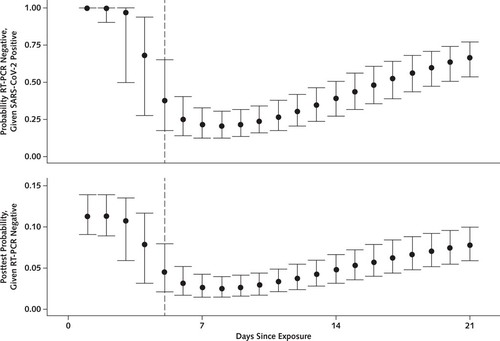
\includegraphics[width=15cm, height=6cm]{Images/RTPCR.jpg}
    %\decoRule
    \caption[RT-PCR Test Negative Rate]{Probability of having a negative RT-PCR test result given SARS-CoV-2 infection (top) and of being infected with SARS-CoV-2 after a negative RT-PCR test result (bottom), by days since exposure \cite{KLL+2020}}
    \label{fig:RT-PCR Test Negative Rate}
    \end{figure}
\vspace{-1em}
Another important factor considering the daily rising numbers are the delays in receiving the results for the RT-PCR test. This places extra strain on the medical professionals in terms of workload and makes it difficult for them to apply safety protocols on suspected patients.

Therefore, due to these aforementioned limitations of the real-time RT-PCR test, finding a safer, more accurate, and faster diagnosis mechanism is essential. Thus, making COVID-19 diagnosis using medical imagery an ideal alternative candidate.

\subsection{Medical Imagery} \label{medical imagery}
Medical Imagery such as X-rays and CT scans have proven to be a viable 
alternative to the RT-PCR test for COVID-19 detection 
due to the limitations mentioned above. The reduced exposure risks, and faster 
diagnosis time are also added benefits.

In this section, CT imaging features of the novel coronavirus 
shall be presented to lay a foundation for future sections 
where we illustrate how deep learning could learn these features 
and use it for automated real-time COVID-19 diagnosis.

A study conducted by Chung et al. on 21 symptomatic  
patients infected with coronavirus admitted to three hospitals in 
three provinces Guangdong, Jiangxi 
and Shandong respectively in China from January 18$^{th}$ 2020 to 
until January 27$^{th}$ 2020 aimed to identify potential imaging 
features of COVID-19 from CT scans reviewed and verified by two fellowship-trained 
cardiothoracic radiologists with approximately 5 years of experience each.

% After evaluation, the following common characteristics were observed:
% \begin{itemize}
%     \item Presence of Ground Glass Opacities (GGO's). 
%     \item Presence of Consolidation. 
%     \item Number of lobes affected by ground-glass or consolidative opacities. 
%     \item Degree of lobe involvement.
%     \item Presence of Nodules.
%     \item Presence of a Pleural Effusion. 
%     \item Presence of Thoracic Lymphadenopathy.
%     \item Presence of underlying lung disease such as Emphysema or Fibrosis.
%     \item Other abnormalities such as Cavitation, Reticulation, Interlobular Septal Thickening, Calcification, and Bronchiectasis.
%   \end{itemize}

The degree of lobe involvement was 
assessed and a "Total Severity Score" was assigned by summing up the each of the 
individual lob scores. Patients were also re-evaluated in order to study the 
progression of features by the same two radiologists \cite{CMA+2020}.

After evaluation, the following common characteristics tabulated in Table \ref{tab:CT Scan Review Results} were observed. Other abnormalities such as Cavitation, Reticulation, Interlobular Septal Thickening, Calcification, and Bronchiectasis were also assessed.
% \vspace{1em}
% The results of the above study are tabulated below: 

\begin{longtable}{| p{.65\textwidth} | p{.163\textwidth} |} 
\hline
\textbf{Finding} & \textbf{No. of Patients} \\
\hline
Ground-glass opacities and consolidation & \\
\quad Absence of both ground-glass opacities and consolidation & 3 (14\%)\\ 
\quad Presence of either ground-glass opacities or consolidation & 18 (86\%)\\
\quad Presence of ground-glass opacities without consolidation & 12 (57\%)\\
\quad Presence of ground-glass opacities with consolidation & 6 (29\%)\\
\quad Presence of consolidation without ground-glass opacities & 0 (0\%)\\ \hline
% No. of lobes affected & \\ \hline
% \quad 0 & 3 (14\%)\\ \hline
% \quad 1 & 1 (5\%)\\ \hline
% \quad 2 & 2 (10\%)\\  \hline
% \quad 3 & 3 (14\%)\\ \hline
% \quad 4 & 4 (19\%)\\ \hline
% \quad 5 & 8 (38\%)\\ \hline
Frequency of lobe involvement & \\ 
\quad Right Upper Lobe & 3 (14\%)\\
\quad Right Middle Lobe & 1 (5\%)\\
\quad Right Lower Lobe & 2 (10\%)\\
\quad Left Upper Lobe & 3 (14\%)\\ 
\quad Left Lower Lobe & 4 (19\%)\\ \hline
% Total lung severity score & \\ \hline
% \quad Mean & 9.9\\ \hline
% \quad Range & 0-19\\ \hline
Opacification distribution and pattern & \\ 
 \quad Rounded Morphology & 7 (33\%)\\ 
 \quad Linear Opacities & 3 (14\%)\\ 
 \quad Crazy-Paving Pattern & 4 (19\%)\\ 
 \quad Peripheral Distribution & 7 (33\%)\\  \hline
More than two lobes affected & 15 (71\%)\\ \hline
Bilateral lung disease & 16 (76\%)\\ \hline
%  \quad Cavitation & 0 (0\%)\\ \hline
%  Other Findings & \\ \hline
%  \quad Discrete Pulmonary Nodules & 0 (0\%)\\  \hline
%  \quad Pleural Effusion(s) & 0 (0\%)\\ \hline
%  \quad Lymphadenopathy & 0 (0\%)\\ \hline
%  \quad Pulmonary Emphysema & 0 (0\%)\\ \hline
%  \quad Pulmonary Fibrosis & 0 (0\%)\\    \hline
 
 \caption{Findings at Initial Chest CT Examination in 21 Patients  \cite{CMA+2020}.}

    \label{tab:CT Scan Review Results}
    \end{longtable}

% The patients with lung severity scores close to the maximum, which was 19, 
% were moved into the intensive care unit. One of the major observations was 
% that besides 3 out of the initial 21 patients, patients were observed to have 
% GGO's or consolidation.
% 
\vspace{-2.7em}
A follow-up chest CT scan was conducted on 8 of the initial 21 patients, within 
a range of 1 to 4 days. Only 1 patient out of the 8 had normal initial and 
follow-up CT scan results. 5 out of eight experienced mild progression in 
the lung characteristics, the remaining 2 displayed 
moderate progression. Fortunately, none of the patients experienced severe progression.

The primary observations from this study on 21 patients include GGO's 
found in 12 patients and consolidation in 6 patients. There is also a high possibility 
the virus affects more than two lobes with bilateral involvement. Other 
observations include rounded morphology detected in 7 patients, 
reticulation in 3 patients, and crazy-paving in 4 patients \cite{CMA+2020}.
% \\
%  \vspace{-2em}

\begin{figure}[H]
 \centering
 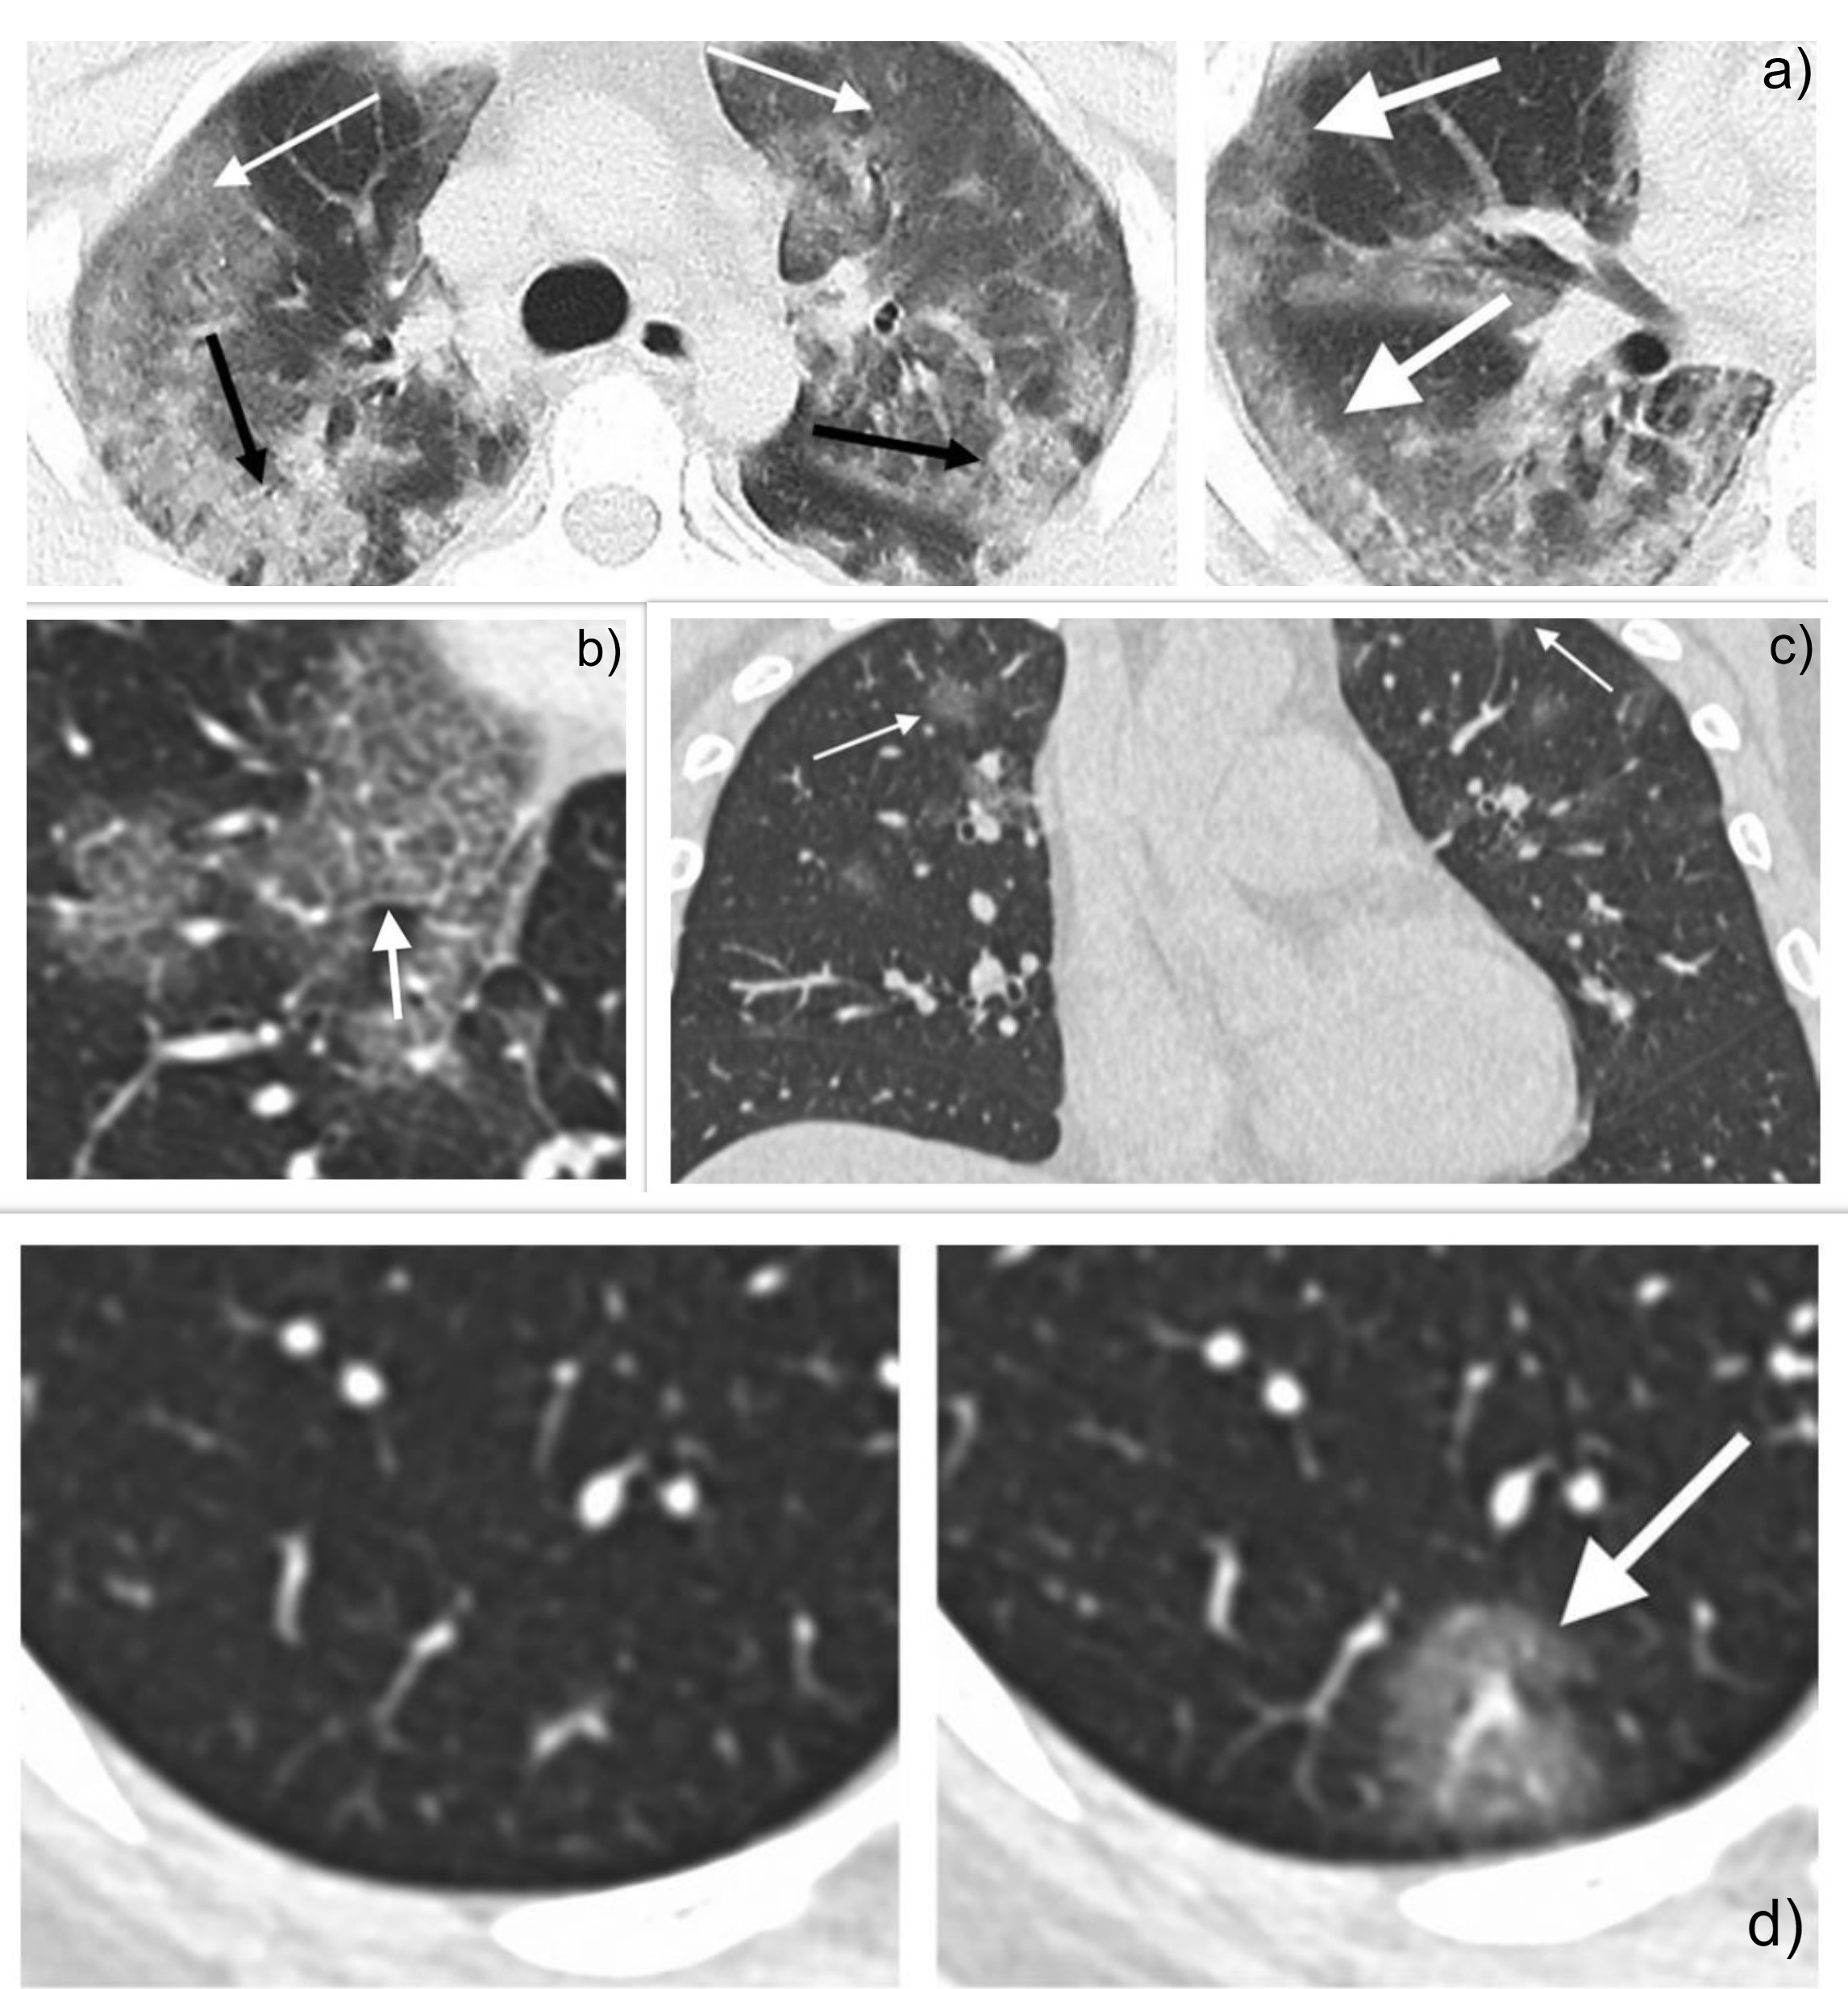
\includegraphics[width=15.5cm, height=12.5cm]{Images/CTScans2.jpg}
 %\decoRule
 \caption[CT Scan Images]{Observed lung CT Scan characteristics. a) White arrow indicates patchy GGO, and black arrow indicates consolidative pulmonary opacities. b) White arrow indicates GGO's with a rounded morphology. c)  White arrow indicates crazy-paving pattern, GGO and interlobular sepal thickening with intralobular lines. d) Follow-up CT scan progression. White arrow indicates new solitary, rounded, peripheral ground-glass lesion \cite{CMA+2020}.}
 \label{fig:CT Scan Image 1}
 \end{figure}
%  \vspace{-2em}
% \begin{figure}[H]
%  \centering
%  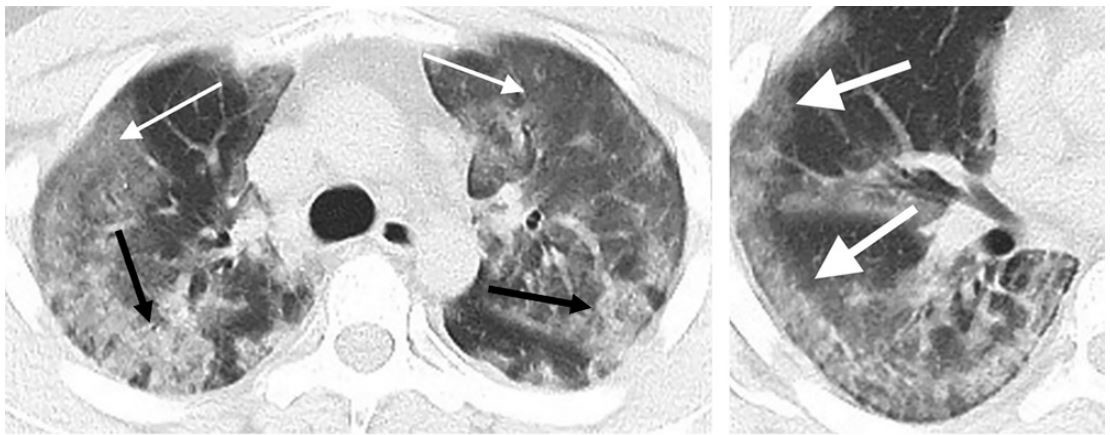
\includegraphics[width=15.5cm, height=5cm]{Images/CTScan1.JPG}
%  %\decoRule
%  \caption[CT Scan Image 1]{Observed lung CT Scan characteristics. White arrow indicates patchy GGO, and black arrow indicates consolidative pulmonary opacities \cite{CMA+2020}.}
%  \label{fig:CT Scan Image 1}
%  \end{figure}

% \begin{figure}[H]
% \centering
% 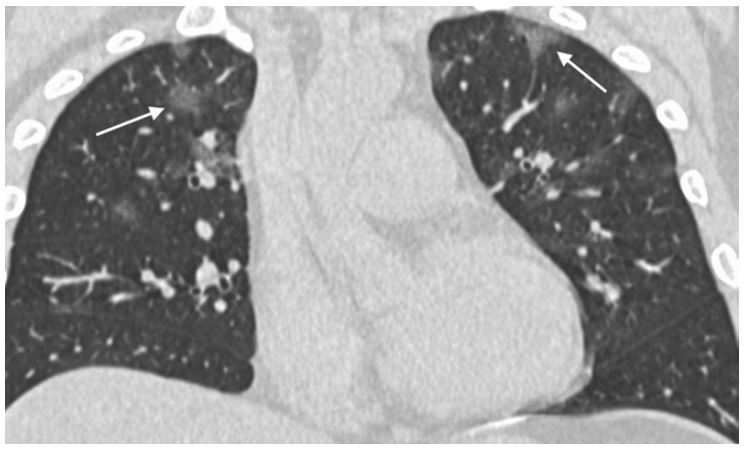
\includegraphics[width=15.5cm, height=5cm]{Images/CTScan2.JPG}
% %\decoRule
% \caption[CT Scan Image 2]{Observed lung CT Scan characteristics. White arrow indicates GGO's with a rounded morphology \cite{CMA+2020}.}
% \label{fig:CT Scan Image 2}
% \end{figure}
        
%  \begin{figure}[H]
%     \centering
%     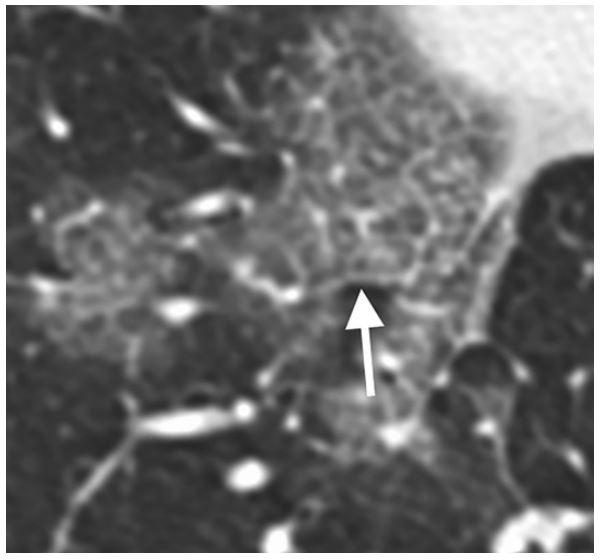
\includegraphics[width=15.5cm, height=5cm]{Images/CTScan3.JPG}
%     %\decoRule
%     \caption[CT Scan Image 3]{Observed lung CT Scan characteristics. White arrow indicates crazy-paving pattern, GGO and interlobular sepal thickening with intralobular lines  \cite{CMA+2020}.}
%     \label{fig:CT Scan Image 3}
%     \end{figure}

% \begin{figure}[H]
%     \centering
%     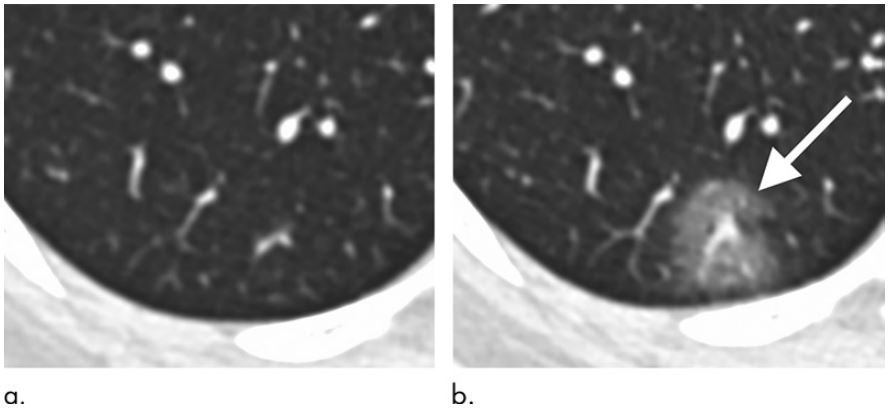
\includegraphics[width=15.5cm, height=6cm]{Images/CTScanProgression.JPG}
%     %\decoRule
%     \caption[CT Scan Progression]{Follow-up CT scan lung characteristics progression. White arrow indicates new solitary, rounded, peripheral ground-glass lesion \cite{CMA+2020}.}
%     \label{fig:CT Scan Image 4}
%     \end{figure}
\vspace{-2em}
One obvious limitation of this study is the relatively low number of 
patients, with only 8 out of 21 carrying out a follow-up CT scan. As this study
was conducted during the dawn of coronavirus, this number is certainly a 
very respective amount.

Another study by Morales et al. whose results are summarized in Appendix \ref{COVID-19 Lung Characteristics}, also observe similar lung characteristics. As we have now seen the prominent imaging characteristics of 
COVID-19, we shall now discuss how deep learning could learn these 
features and accurately diagnose patients with COVID-19 in real-time. 

\section{Deep Learning for COVID-19 Diagnosis}

The coronavirus global pandemic spreading rapidly all across the world have 
forced scientists and researchers to identify alternative 
diagnosis mechanisms in addition to the RT-PCR test to overcome 
its limitations. As we have seen in previous sections, 
medical imagery such as X-rays and CT scans have played a 
vital role in combating the rising numbers by saving 
valuable time in diagnosis and reducing virus exposure.

Deep learning techniques have further enhanced COVID-19 diagnosis 
using medical imagery due to its rapid detection capabilities, 
fully automated and efficient diagnosis workflow, 
and assisting medical practitioners by highlighting observed 
COVID-19 lung characteristics similar to 
features discussed in the section \ref{medical imagery}. A detailed overview of the modern CT and X-ray systems enabling automated diagnosis workflow ensuring minimal virus exposure can be found in Appendix \ref{Automated Diagnosis Workflow}.

% In this section, we will have a comprehensive discussion on how 
% deep learning techniques could accurately diagnose patients with COVID-19 by reviewing the methodologies used and the results 
% obtained by experiments and studies conducted across the world.

To identify the regions of interest (ROIs), segmentation of the 
lung CT or X-ray scans are a vital pre-requisite. The former produces 
high-quality 3D images for detecting COVID-19 whereas the latter involves 
the ribs being projected onto soft-tissues in 2D. 

As a result, segmentation 
in X-ray scans is more challenging as compared to CT scans. But on the other hand, 
X-ray scans are more widely accessible in medical facilities all across the world 
and are usually the first imaging modality used on patients suspected of COVID-19.

Keeping in mind these limitations, the next two subsections review the segmentation techniques using deep learning for both CT and X-rays respectively and 
discuss the results obtained.

\subsection{CT Based Diagnosis of COVID-19}
To identify the ROIs from a CT scan for diagnosis, deep learning 
techniques are extensively used. These techniques could be narrowed down 
to the three most prominent segmentation methods which are \textbf{U-Net} \cite{CXZ+2020, CYZ+2020, HLR+2020, YHQ+2020, GOM+2020, LLL+2020}, \textbf{UNet++} \cite{CJL+2020, JSB+2020}, and \textbf{VB-Net}  \cite{SFY+2020} respectively.

% \begin{itemize}
%     \item U-Net \cite{CXZ+2020, CYZ+2020, HLR+2020, YHQ+2020, GOM+2020, LLL+2020}
%     \item UNet++ \cite{CJL+2020, JSB+2020}
%     \item VB-Net \cite{SFY+2020}
% \end{itemize}

From section \ref{medical imagery}, we can infer that the main ROIs could be classified into 
two specific categories, which are lung-region and lung-lesion oriented 
methods. The latter is more of a challenge in terms of its detection as lesions 
could be in a variety of shapes and sizes, furthermore, locating its region 
also adds to the difficulty in identifying it.

The literature indicates U-Net architecture as most reliable in segmenting both lung regions and lesions in COVID-19 diagnosis 
applications. Designed by Ronneberger, U-Net as its name suggests has a U-shape architecture, 
such that it has a symmetric expansive and contracting path \cite{RFT2015}.

\begin{figure}[H]
    \centering
    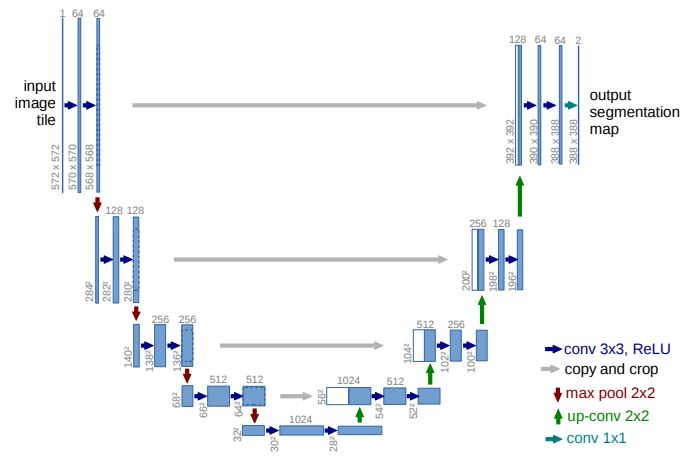
\includegraphics[height=6.5cm]{Images/UNet.JPG}
    %\decoRule
    \caption[U-Net Architecture]{A representation of the U-Net architecture \cite{RFT2015}}
    \label{fig:U-Net Architecture}
    \end{figure}
\vspace{-2em}
Various variants of the U-Net have been developed since its inception due to its high ability to learn visual semantics and therefore are suitable 
for many medical applications. They include the following:
\begin{itemize}
    \item \textbf{3D U-Net} - Replaces the conventional U-Net layers with 3D layers. \cite{SCS+2020}
    \item \textbf{V-Net} - Utilizes residual blocks as the convolutional block, network optimization carried out through Dice Loss. \cite{MNA+2020}
    \item \textbf{VB-Net} - Combination of V-Net with a bottle-neck structure. \cite{SFY+2020}
    \item \textbf{UNet++} - A more complex version of U-Net, inserts a nested convolutional structure between the expansive and contracting path. \cite{ZSM+2020}
    \item \textbf{Attention U-Net} - Integrates Attention Gates with U-Net architecture to focus on target structures of various shapes and sizes. \cite{OSF+2020}
\end{itemize}

% \vspace{-2em}
Identifying and labeling the training data for the purpose of COVID-19 diagnosis is often 
time consuming and labour intensive, especially the manual detection of lesions. Shan et al. proposes a workaround which involves the "human-in-the-loop" strategy, 
where radiologists play an integral part in the training process \cite{SFY+2020}. Another similar suggestion from Yue et al. was to allow the radiologists to provide initial seeds for the U-Net  model \cite{YHQ+2020}.

Zheng et al. suggests an alternative approach, where unsupervised methods are used to generate pseudo segmentation masks for images to overcome 
the labeling process and thus avoid its limitations. In addition to reviewing results of lung segmentation from the U-Net model, Zheng et al. also utilizes a 3D CNN to predict the probability of 
COVID-19 using images obtained as an input \cite{CXZ+2020}. With a 
dataset of 540 patients, 313 with COVID-19, and remaining without COVID-19 
are used for training and testing purposes. The model attains a sensitivity 
of 90.7\% and specificity 91.1\%.

The lung segmentation's obtained could be used for COVID-19 diagnosis and for the 
quantification of data. The literature mentioned in this section includes both of the 
objectives.

Li et al. conducted a multi-center study by distinguishing COVID-19 from community-acquired pneumonia \cite{LLL+2020}. A combination of U-Net and ResNet-50 was proposed with the former used to extract lung regions using pre-processed 2D slices. The latter along with shared weights between the 2D slices combined 
with max-pooling is used for COVID-19 diagnosis. This study utilizes a large dataset 
with 1296 COVID-19 patients, 1735 with community-acquired pneumonia, and 1325 
non-pneumonia patients. The model achieves a specificity of 96\% and sensitivity 
of 90\%.  

An AI system developed by Jin et al. for rapid COVID-19 diagnosis, involves the input to the classification model 
being the CT slices which have been segmented \cite{JSB+2020}. Instead of a 3D CNN, a ResNet-50 model was used for diagnosis
and UNet++ for lung segmentation and lesion identification. The model 
is trained on 1136 images, 723 COVID-19 positives, and 413 negatives and 
achieves sensitivity and specificity of 97.4\% and 92.2\% respectively.

As for the quantification of data, both Cao et al. \cite{CYZ+2020} and Huang et al. \cite{HLR+2020} monitor the longitudinal 
progression of COVID-19 using the CT segmentation of pulmonary opacities using the segmentation of 
the lung region and GGO. Therefore, the image segmentation obtained aids radiologists 
in infection identification, analysis, and diagnosis.

Most of the classification studies involve segregating COVID-19 patients 
from non-COVID-19 with most of the latter patients being segregated further 
into pneumonia and non-pneumonia subjects.

Chen et al. developed a UNet++ model which segments lung lesions 
\cite{CJL+2020} using CT images of 51 COVID-19 patients and 
55 patients with other diseases and diagnose patients with 95.2\% accuracy thus reducing the reading time of radiologists by 65\%. Given 
raw images to the model, prediction boxes displaying suspected regions were output,
after further extraction and filtering a logic linking of predictions was added, which 
aimed to aid radiologists in manual detection of the virus.

Jin et al. considers an alternative approach  
utilizing 2D Deeplab v1 and 2D ResNet-152 models for lung segmentation 
and lung-mask slice based classification of COVID-19 respectively \cite{JCW+2020}. The 
model achieves a respectable score of 94.1\% sensitivity and 95.5\% 
specificity using a dataset of 496 COVID-19 positive CT scan images.

The objective of the remaining studies besides COVID-19 diagnosis is its differentiation
with common pneumonia which primarily 
includes viral pneumonia. The main reason for this objective being the 
very similar radiological appearances of both the diseases.

Wang et al. classifies between COVID-19 and viral pneumonia using a 2D CNN model on delineated 
region patches \cite{WBX+2020}. Experiments were conducted on chest CT scans from 
44 COVID-19 and 55 pneumonia patients with external testing 
resulting in 79.3\% accuracy.

Experiments carried out by Song et al. employs OpenCV to segment 
2D slices which include lung regions \cite{SZL+2020}. The 3D chest CT images resulted in 
15 2D slices of complete lungs and each slice were fed into the deep learning based CT diagnosis system also called DeepPneumonia. A combination of 
a pre-trained ResNet-50 along with Feature Pyramid Network (FPN) which can 
extract specific ranked details from the images, coupled 
with an attention module to learn these extracted details were used to develop this model.

The dataset includes 88 COVID-19 patients, 101 bacterial pneumonia and 86 
healthy patients. The proposed model achieves a classification accuracy of 86\%.

Table \ref{tab:CT Image Segmentation Techniques} and \ref{tab:COVID-19 Diagnosis Applcations} summarizes all the COVID-19 image segmentation 
applications mentioned in this section,
and the results of diagnosis experiments conducted across various 
medical facilities. An extended version of Table \ref{tab:CT Image Segmentation Techniques} can be found in Appendix \ref{CT Image Segmentation Techniques}.
\vspace{1em}

\begin{longtable}{| p{.25\textwidth} | p{.15\textwidth} |  p{.25\textwidth} |} 

    \hline
\textbf{Study} & \textbf{Method} & \textbf{Target ROI}  \\
\hline
\multirowcell{2}{Zheng et al. \cite{CXZ+2020}} & \multirowcell{2}{U-Net} & \multirowcell{1}{Lung} \\ \cline{3-3}  & & \multirowcell{1}{Lesion}  \\ \hline
\multirowcell{2}{Cao et al. \cite{CYZ+2020}} & \multirowcell{2}{U-Net} &  \multirowcell{1}{Lung} \\ \cline{3-3} & & \multirowcell{1}{Lesion} \\ \hline
\multirowcell{3}{Huang et al. \cite{HLR+2020}} & \multirowcell{3}{U-Net} & \multirowcell{1}{Lung} \\ \cline{3-3} & & \multirowcell{1}{Lung Lobes} \\ \cline{3-3} & &  \multirowcell{1}{Lesion}  \\ \hline
\multirowcell{2}{Yue et al. \cite{YHQ+2020}} & \multirowcell{2}{U-Net} & \multirowcell{1}{Lung Lobes} \\ \cline{3-3} & & \multirowcell{1}{Lesion} \\ \hline
\multirowcell{2}{Gozel et al. \cite{GOM+2020}} & \multirowcell{2}{U-Net} & \multirowcell{1}{Lung} \\ \cline{3-3}  & & \multirowcell{1}{Lesion} \\ \hline
% \multirowcell{4}{Shan et al. \cite{SFY+2020}} & \multirowcell{4}{VB-Net} & \multirowcell{4}{Diagnosis} & \multirowcell{1}{Lung} \\ \cline{4-4} & & & \multirowcell{1}{Lung Lobes} \\ \cline{4-4} &  & & \multirowcell{1}{Lung Segments} \\ \cline{4-4} & & & \multirowcell{1}{Lesion}\\ \hline
% \multirowcell{1}{Li et al. \cite{LLL+2020}} & \multirowcell{1}{U-Net} & \multirowcell{1}{Diagnosis} & \multirowcell{1}{Lesion} \\ \hline
% \multirowcell{1}{Chen et al. \cite{CJL+2020}} & \multirowcell{1}{UNet++} & \multirowcell{1}{Diagnosis} & \multirowcell{1}{Lesion} \\ \hline
% \multirowcell{2}{Jin et al. \cite{JSB+2020}} & \multirowcell{2}{UNet++} & \multirowcell{2}{Diagnosis} & \multirowcell{1}{Lung} \\ \cline{4-4} & & &  \multirowcell{1}{Lesion}\\ \hline
\multirowcell{4}{Tang et al. \cite{TLX+2020}} & \multirowcell{4}{Commercial\\Software} & \multirowcell{1}{Lung} \\ \cline{3-3}  & & \multirowcell{1}{Lesion} \\ \cline{3-3}  & & \multirowcell{1}{Trachea} \\ \cline{3-3}  & & \multirowcell{1}{Bronchus}\\ \hline
% \multirowcell{3}{\cite{SCN+2020}} & \multirowcell{3}{Threshold-based\\Region Growing\\\cite{LBC+2020}} & Lesion \\ \hline

\caption{CT Image Segmentation Techniques in COVID-19 Quantification Applications \cite{SFJ+2020}}

    \label{tab:CT Image Segmentation Techniques}
    \end{longtable}
    
% \vspace{-1em}

\begin{longtable}{| p{.25\textwidth} | p{.20\textwidth} | p{.15\textwidth} | p{.20\textwidth} |} 

    \hline
\textbf{Study} & \textbf{Subjects} & \textbf{Method} & \textbf{Result}  \\
\hline
\multirowcell{2}{Zheng et al. \cite{CXZ+2020}} & \multirowcell{1}{313 COVID-19} & \multirowcell{1}{U-Net} & \multirowcell{1}{90.7\% (Sens.)} \\ \cline{2-4} & \multirowcell{1}{229 Others} & \multirowcell{1}{CNN} & \multirowcell{1}{91.1\% (Spec.)}\\ \hline
\multirowcell{3}{Li et al. \cite{LLL+2020}} & \multirowcell{1}{468 COVID-19} & \multirowcell{3}{ResNet-50} & \multirowcell{1}{90.0\% (Sens.)} \\ \cline{2-2} \cline{4-4}  & \multirowcell{1}{1551 CAP} & & \multirowcell{1}{96.0\% (Spec.)} \\ \cline{2-2} \cline{4-4} & \multirowcell{1}{1445 Non-pneu.} && \multirowcell{1}{0.95 (AUC.)}\\ \hline
\multirowcell{2}{Chen et al. \cite{CJL+2020}} & \multirowcell{1}{51 COVID-19} & \multirowcell{2}{UNet++} & \multirowcell{1}{100\% (Sens.)} \\ \cline{2-2} \cline{4-4} & \multirowcell{1}{55 Others} &  & \multirowcell{1}{93.6\% (Spec.)} \\ \hline
\multirowcell{2}{Jin et al. \cite{JSB+2020}} & \multirowcell{1}{723 COVID-19} & \multirowcell{2}{UNet++} & \multirowcell{1}{97.4\% (Sens.)} \\ \cline{2-2} \cline{4-4} & \multirowcell{1}{413 Others} &  & \multirowcell{1}{92.2\% (Spec.)} \\ \hline
\multirowcell{2}{Jin et al. \cite{JCW+2020}} & \multirowcell{1}{496 COVID-19}& \multirowcell{2}{CNN} & \multirowcell{1}{94.1\% (Sens.)} \\ \cline{2-2} \cline{4-4} & \multirowcell{1}{1385 Others} &  & \multirowcell{1}{95.5\% (Spec.)} \\ \hline
\multirowcell{3}{Song et al. \cite{SZL+2020}} & \multirowcell{1}{88 COVID-19} & \multirowcell{3}{ResNet-50} & \multirowcell{3}{86.0\% (Acc.)} \\ \cline{2-2}  & \multirowcell{1}{100 Bac. Pneu.} &  & \\ \cline{2-2}  & \multirowcell{1}{86 Normal} &  & \\ \hline
\multirowcell{2}{Wang et al. \cite{WBX+2020}} & \multirowcell{1}{44 COVID-19} & \multirowcell{2}{CNN} & \multirowcell{2}{79.3\% (Acc.)} \\ \cline{2-2} & \multirowcell{1}{55 Vir. Pneu.} &  & \\ \hline
\caption{COVID-19 Diagnosis Applications and their results from CT Image Segmentation \cite{SFJ+2020}}
\label{tab:COVID-19 Diagnosis Applcations}
    \end{longtable}
\begin{center} 
\vspace{-2em}
\textcolor{red}{* } Bac. - Bacterial, Vir. - Viral, Pneu. - Pneumonia \end{center}
As we have seen, the above studies result in promising diagnosis outcomes. Therefore, 
COVID-19 diagnosis with CT images could facilitate early detection of the coronavirus 
and also reduce the high exposure rates between patients and medical professionals.

\subsection{X-ray Based Diagnosis of COVID-19}
X-rays are most often the first imaging modality used on suspected patients, due 
to its wide availability in most clinics and medical facilities. As seen in section \ref{medical imagery},
radiological signs include GGOs, consolidation, and opacification.

In order to detect these abnormalities in lung X-ray scans, three popular 
architecture's are used across various studies which are \textbf{ResNet} \cite{ZXS+2020}, \textbf{ResNet-50} \cite{AKP2020}, and \textbf{CNN} \cite{GHT2020, LWA2020}.
% \vspace{-2em}
% \begin{itemize}
%     \item ResNet \cite{ZXS+2020}
%     \item ResNet-50 \cite{AKP2020}
%     \item CNN \cite{GHT2020, LWA2020}
% \end{itemize}
% \vspace{-2em}

\begin{figure}[H]
    \centering
    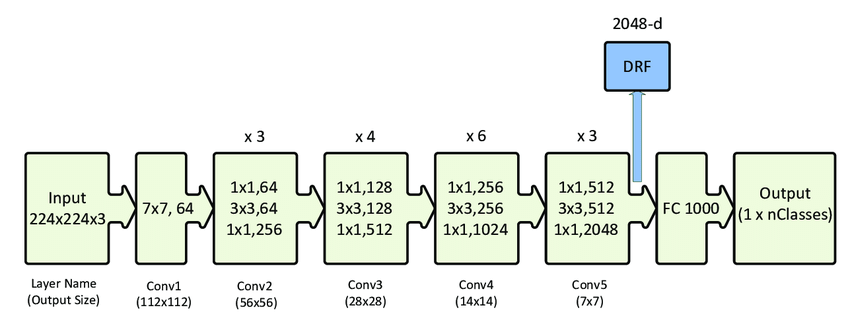
\includegraphics[width=15cm, height=3.5cm]{Images/ResNet.png}
    %\decoRule
    \caption[ResNet-50 Architecture]{ResNet-50 architecture with residual units \cite{MOB+2020}}
    \label{fig:ResNet-50 Architecture}
    \end{figure}
\vspace{-2em}
X-rays despite, as mentioned previously, being the first imaging modality for 
patients suspected with COVID-19 is less sensitive than 3D chest CT images. 
Anomalous chest radiographs are found in 69\% of the patients initially during 
admission and this number increases to 80\% after a certain period 
once hospitalized \cite{WLA+2020}.

To estimate the uncertainty in COVID-19 prediction Ghoshal et al. \cite{GHT2020} proposes 
a Bayesian CNN. X-rays of 70 COVID-19 patients are obtained 
from Cohen et al. \cite{JMD2020} and others from Kaggle's chest X-ray images. Bayesian 
inference improves the detection accuracy of the model from 85.7\% to 92.9\% from 
the experiments conducted by the authors.

Narin et al. experiments with three deep learning models 
i.e., ResNet-50, InceptionV3 and Inception-ResNetV2 respectively, with the objective 
to detect COVID-19 from X-ray images  \cite{AKP2020}. The dataset includes X-rays from 50 COVID-19 patients and 50 normal scans.
 The results indicate that ResNet-50 achieves highest accuracy with 98\% followed by InceptionV3 which 
attains 97\%.

Zhang et al. also suggest a ResNet based model for COVID-19 detection \cite{ZXS+2020}. 
But the model aims to achieve two objectives, one for COVID-19 classification and another for anomaly detection. The experiment was conducted on a dataset containing X-rays from 
70 COVID-19 patients and 1008 other X-rays. The anomaly detection score in-turn optimizes the COVID-19 
classification score which reaches 96\% from the experiments conducted by the authors.

Wang et al. proposes a deep CNN based model (COVID-Net) and
achieves a testing accuracy of 83.5\%  \cite{LWA2020}. The dataset used for the study include X-rays from 
patients diagnosed with both Bacterial and Viral Pneumonia. More specifically, 
45 COVID-19 positive, 931 Bacterial Pneumonia, 660 Viral Pneumonia, and 1203 normal X-rays.

Table \ref{tab:X-ray Image Segmentation Techniques} summarizes the results obtained by the experiments discussed in this section.
% \\
\begin{longtable}{| p{.30\textwidth} | p{.20\textwidth} | p{.15\textwidth} | p{.15\textwidth} |} 

    \hline
\textbf{Study} & \textbf{Subjects} & \textbf{Method} & \textbf{Result}  \\
\hline
\multirowcell{2}{Ghoshal et al. \cite{GHT2020}} & \multirowcell{1}{70 COVID-19} & \multirowcell{2}{CNN} & \multirowcell{2}{92.9\% (Acc.)} \\ \cline{2-2} & \multirowcell{1}{Others} & &\\ \hline
\multirowcell{2}{Zhang et al. \cite{ZXS+2020}} & \multirowcell{1}{70 COVID-19} & \multirowcell{2}{ResNet} & \multirowcell{1}{96.0\% (Sens.)} \\ \cline{2-2} \cline{4-4} & \multirowcell{1}{1008 Others} &  &  \multirowcell{1}{70.7\% (Spec.)} \\ \hline
\multirowcell{2}{Narin et al. \cite{AKP2020}} & \multirowcell{1}{50 COVID-19} & \multirowcell{2}{ResNet-50} & \multirowcell{2}{98.0\% (Acc.)} \\ \cline{2-2} & \multirowcell{1}{50 Normal} & &\\ \hline
\multirowcell{4}{Wang et al. \cite{LWA2020}} & \multirowcell{1}{45 COVID-19} & \multirowcell{4}{CNN} & \multirowcell{4}{83.5\% (Acc.)} \\ \cline{2-2} & \multirowcell{1}{931 Bac. Pneu.} &  & \\ \cline{2-2} &  \multirowcell{1}{660 Viral Pneu.} && \\  \cline{2-2} &  \multirowcell{1}{1203 Normal} && \\ \hline
\caption{X-ray Image Segmentation Techniques in COVID-19 Diagnosis Applications \cite{SFJ+2020}}

    \label{tab:X-ray Image Segmentation Techniques}
    \end{longtable}
\vspace{-2em}
\begin{center}\textcolor{red}{* } Acc. - Accuracy, Sens. - Sensitivity, Spec. - Specificity \end{center}

As seen in the above studies on X-ray images, the classification of COVID-19 from other Pneumonia seems 
to be a repeating objective. The major limitation involves the lack of data available as 
currently there exist two online datasets with 70 images from COVID-19 patients, therefore 
the generalizability and stability of the model are yet to be evaluated.

\subsection{Interpreting Deep Learning Results}
\label{Interpreting Deep Learning Results}
Deep learning techniques are often regarded as "Black Boxes" concerning 
its training and classification mechanisms. In medical applications such as this topic where we 
aim to diagnose patients with COVID-19 in real-time, understanding the reasoning behind the model's prediction 
is of utmost importance. 

More than just an additional insight, visualization of distinct features 
from the lung segmentation images would allow radiologists to cross-check their findings with that of the deep 
learning model and thus allow for an even better and reliable diagnosis.

Saliency methods are a set of popular and powerful tools which allow researchers 
to analyze and understand deep learning decisions \cite{AGM+2018}. 
Various interpretation methods exist in deep learning with a few of them 
mentioned below:
\begin{itemize}
    \item \textbf{Saliency Map} - Estimates specific parts of the image which contributes to highest layer activation \cite{ZMF2013}.
    \item \textbf{Class Activation Mapping (CAM)} - Averages and adds the activation's of each feature map (Global Average Pooling) and uses this to highlight important regions \cite{ZKL+2015}.
    \item \textbf{Gradient-Weighted CAM (Grad-CAM)} - Calculates the gradient of the classification score with respect to the convolutional features \cite{RCD+2017}.
\end{itemize}

The saliency maps shown in Figure \ref{fig:X-ray images and their corresponding heat maps} and \ref{fig:Saliency Maps displaying COVID-19 lung characteristics in CT and X-ray scans} highlight those regions in the lungs 
which as discussed in Section \ref{medical imagery}, exhibit the most common characteristics 
in patients diagnosed with COVID-19. 
GGO's, consolidations, lesions, and crazy-paving patterns are some of the 
more contributing features for diagnosis purposes by the 
deep learning model as indicated by the saliency maps.

    \begin{figure}[H]
    \centering
    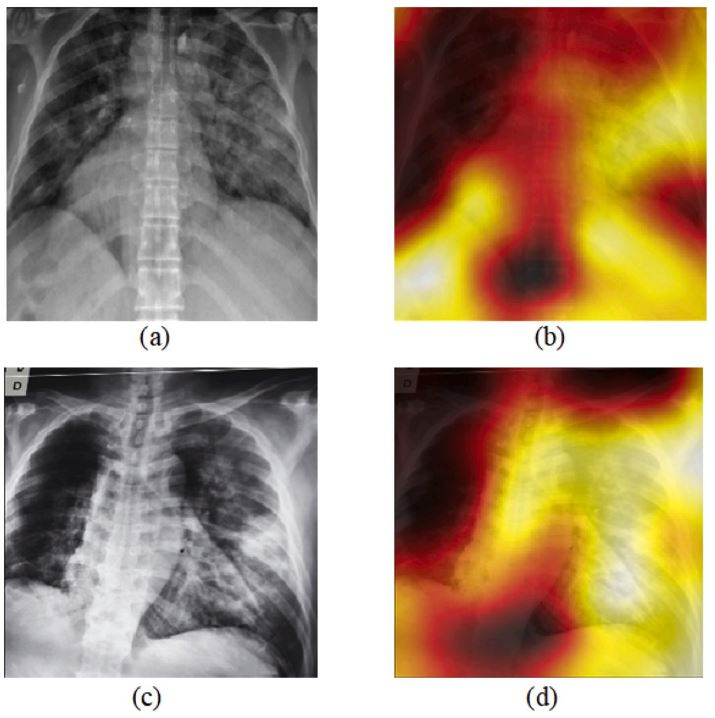
\includegraphics[width=15cm, height=6cm]{Images/Saliency4.JPG}
    %\decoRule
    \caption[X-ray Heat Map]{X-ray images and the corresponding heat maps \cite{OTY+2020}}
    \label{fig:X-ray images and their corresponding heat maps}
    \end{figure}




% Below shown are some saliency maps observed across multiple studies:
\begin{figure}[H]
    \centering
    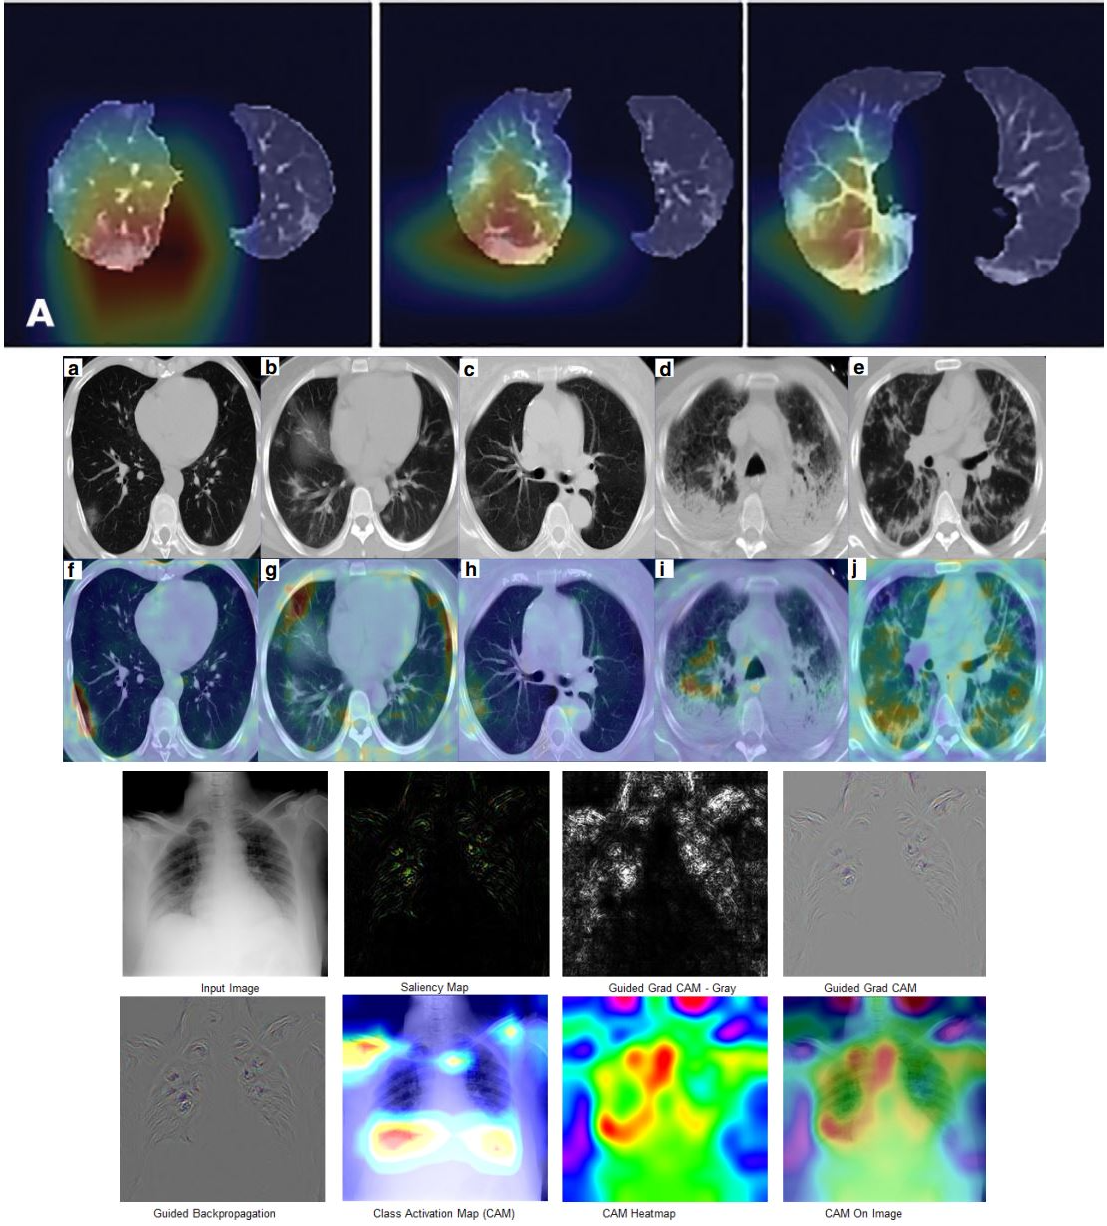
\includegraphics[width=15.5cm, height=12cm]{Images/Saliency Maps.png}
    %\decoRule
    \caption[Attention Heat Map]{Saliency Maps displaying COVID-19 lung characteristics in CT and X-ray scans \cite{LLL+2020} \cite{GHT2020} \cite{HSX+2020}}
    \label{fig:Saliency Maps displaying COVID-19 lung characteristics in CT and X-ray scans}
    \end{figure}
    

\vspace{-2em}
% \begin{figure}[H]
%     \centering
%     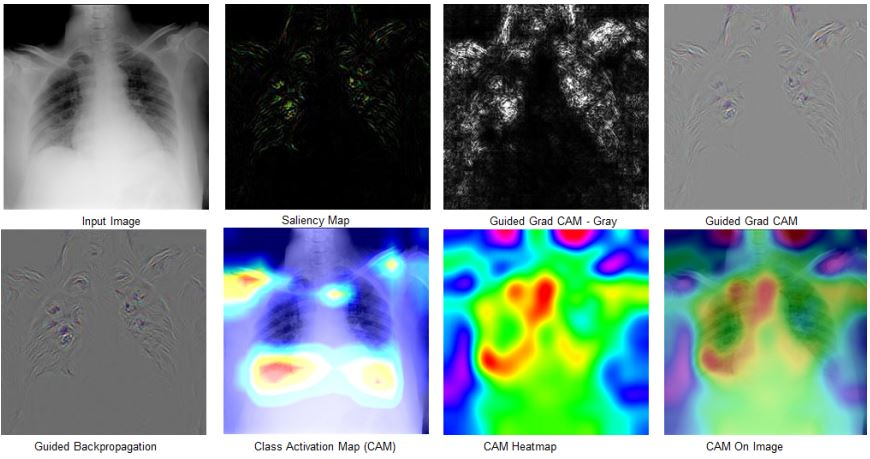
\includegraphics[width=15cm, height=5.5cm]{Images/Saliency.JPG}
%     %\decoRule
%     \caption[X-ray Saliency Map]{Saliency Map displaying COVID-19 lung characteristics in X-rays \cite{GHT2020}}
%     \label{fig:Saliency Map displaying COVID-19 lung characteristics in X-rays}
%     \end{figure}

%     \begin{figure}[H]
%         \centering
%         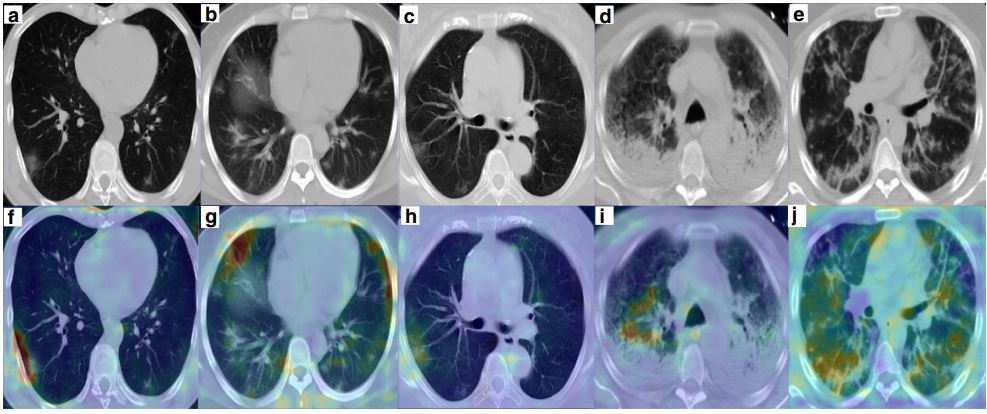
\includegraphics[width=15cm, height=5.5cm]{Images/Saliency2.JPG}
%         %\decoRule
%         \caption[CT Scan Saliency Map]{Saliency Map displaying COVID-19 lung characteristics in CT scans \cite{HSX+2020}}
%         \label{fig:Saliency Map displaying COVID-19 lung characteristics in CT scans}
%         \end{figure}

% The saliency maps highlight those regions in the lungs 
% which as discussed above, exhibit the most common characteristics 
% in patients diagnosed with COVID-19. 
% GGO's, consolidations, lesions, and crazy-paving patterns are some of the 
% more contributing features for diagnosis purposes by the 
% deep learning model as indicated by the saliency maps.

The results of saliency maps are therefore, in direct 
correlation with studies shown above which displays 
the most repeating COVID-19 lung characteristics. This provides 
additional assistance and assurance to radiologists who during 
diagnosis, look to identify the same lung characteristics.

% \vspace{-1em}
\section{Discussion}
The integration of AI techniques in medical research has 
just scratched the surface. We have discussed many studies 
which have experimented on fully automated COVID-19 
diagnosis employing deep learning methods and have 
yielded respectable results. But as mentioned, this is 
only the beginning and medical industry is due for a 
breakthrough soon. 

% \vspace{-1em}
\subsection{Overview of COVID-19 Applications}

Among many medical applications, where AI could potentially 
optimize and improvise standard procedures, automated 
imaging acquisition workflows as discussed previously, seem to be at the forefront. The overall efficiency of scanning procedure 
whether it be CT or X-rays could be enhanced and as a direct result, 
exposure to transferable viruses such as the coronavirus could be 
decreased, thus protecting medical professionals. 

% Besides protecting medical professionals, reducing patient 
% exposure to X-rays is also important. Calculating the right amount of radiation 
% to be used via body region thickness of the patient, finding an optimal patient position without technician intervention by automated calculation of 
% scan range and centering are promising AI-empowered solutions.

Section \ref{Interpreting Deep Learning Results} discusses Class Activation Mapping (CAM) which is a conventional 
technique to focus on prominent pixels or regions which lead to a 
resultant classification. Studies which have utilized this technique 
for COVID-19 diagnosis have seen a close correlation between the patterns 
identified by radiologists and the regions highlighted by the model therefore 
ensuring the reliability of the predictions given by the model.

Explainable Artificial Intelligence (XAI) methods \cite{ADD+2020, FSA+2020} are a recent addition 
to deep learning interpretability techniques which provides a finer localization 
map and exhibits more intricate details when compared to 
Class Activation Mapping (CAM) techniques.
% \vspace{-1em}
\subsection{Critical Review}

Using medical imagery for disease diagnosis has variety of applications, for example, 
diagnosing COVID-19 as seen through experiments conducted by multiple studies. But one noticeable caveat is the observed negative radiological signs during preliminary stages of the disease. This could have critical consequences in real-life circumstances especially amid a global pandemic.

% Overfitting of the results is very common in medical applications due to the lack of data available. Studies that involve AI techniques for segmentation and disease diagnosis are often hampered by this limitation. Therefore, to generalize the results obtained from a study, the availability of a respectable number of data is essential.

Many studies mentioned above use U-Net architecture for lung segmentation and variants of CNN's such as ResNet and ResNet-50 for COVID-19 diagnosis. One of the limiting factors of AI-based experiments is the difficulty in extracting the reasons as to why the deep learning model resulted in a certain classification. 

COVID-19 applications employing deep learning often require accurate 
labeling of data, but this task often is very time-consuming and medical 
professionals due to the rising numbers often would not be able to carry out 
this procedure. This leads to incomplete and inaccurate labeling of data which 
proves to be an additional challenge to deep learning models who train on this 
dataset and therefore result in an incorrect diagnosis.

Exploiting unsupervised training techniques \cite{NVF+2018, DGE2015} or exploring transfer learning methods \cite{TFK+2018}
where filters applied on a completely different dataset could be 
reused for COVID-19 applications are viable options to mitigate the above labeling 
complication.

As the coronavirus was declared a global pandemic fairly recently in early 2020, limited 
follow-up studies exist to identify treatment mechanisms and 
evaluating diagnosis tools. Few studies such as from Chung et al. \cite{CMA+2020}, mentioned earlier 
did in fact carry out follow-up CT scans to recognize progression patterns from 
segmented lung images, but due to the lack of participants when compared to the 
the initial version, the results obtained could not be reliably applied in the real world.

% Applying the findings obtained and methods carried out from 
% experiments conducted on related studies similar to COVID-19 diagnosis 
% would be the ideal path to take during this stage of the pandemic. 
% Especially from various pneumonia diseases as we have seen earlier to have similar radiological observations as that of the coronavirus. Deep learning 
% techniques employed for the diagnosis of pneumonia could also be replicated for 
% COVID-19 diagnosis.

% Applying the findings obtained and methods carried out from 
% experiments conducted on related studies similar to COVID-19 diagnosis 
% would be the ideal path to take during this stage of the pandemic. 
Tracking of COVID-19 patients is essential for containing 
the spread of the virus. Therefore medical facilities should enforce 
strict patient follow-up protocols carrying out long-term monitoring and capturing 
progression data which could be used by studies to further develop their models 
and deploy them in the real world. 

% \vspace{-1em}
\section{Conclusion and Research Questions}
The coronavirus has affected millions of lives throughout the world. 
Front-line workers combat the virus tirelessly to counter 
the rapidly rising numbers daily. In this chapter, we have discussed 
how deep learning could provide a safe, efficient and accurate 
workflow for COVID-19 diagnosis and be a suitable alternative to 
the RT-PCR test.

% AI-empowered techniques starting with automated scanning workflow 
% with the objective of reducing virus and radiation exposure for 
% the technicians and patients respectively, followed by two prominent 
% imaging modalities, i.e., CT and X-ray could play a pivotal role in 
% COVID-19 diagnosis.

It is important to couple the results obtained 
using the same imaging workflow discussed in this chapter, with clinical 
observations and laboratory results to provide reliable COVID-19 diagnosis.
From the experiments and studies discussed, it is safe to conclude 
that AI if utilized effectively could play a vital role in 
accurate diagnosis and analysis of COVID-19, and therefore potentially 
save precious lives and ultimately lead to our victory against the coronavirus
global pandemic.
\vspace{-1em}
\subsection*{Research Questions}
Based on the gaps we identified in this chapter, we plan to answer the following research questions:
%Upon project completion we aim to find answers to the following questions after applying  suitable evaluation strategies:

\begin{enumerate}
  \item Is there a correlation between the ROIs detected by the deep learning model and the lung characteristics observed on COVID-19 patients?
  \item Are the results obtained by the deep learning approach better when compared to the standard RT-PCR test?
  \item Is it feasible to deploy and utilize the deep learning model in medical facilities and laboratories for rapid real-time COVID-19 diagnosis?
\end{enumerate} 
% Chapter Template

\chapter{Requirements Analysis and Evaluation Strategy} % Main chapter title
\label{Requirements Analysis}
\label{ChapterX} % Change X to a consecutive number; for referencing this chapter elsewhere, use \ref{ChapterX}

%----------------------------------------------------------------------------------------
%	SECTION 1
%----------------------------------------------------------------------------------------

This chapter provides an insight into the project requirements followed by demonstrating the project implementation workflow, UI wireframe, data collection, and processing methodology, and concludes with an evaluation strategy.

\section{Requirements Analysis}
This section identifies and outlines the functional and non-functional requirements pertaining to this project. The priority 
of each of these requirements are ranked according to the MSCW prioritization technique. The following color-scheme 
indicates the respective ranking order:

\begin{itemize}
  \item \colorbox{green}{\textbf{Must Have (M)}} - These requirements are fundamental to achieve the aim of this project.
  \item \colorbox{cyan}{\textbf{Should Have (S)}} - These requirements are important to the project but not vital and could be achieved in the long run.
  \item \colorbox{yellow}{\textbf{Could Have (C)}} - These requirements are not fundamental to achieve the aim of this project but would be an added benefit if accomplished.
  \item \colorbox{pink}{\textbf{Want To Have (W)}} - These requirements would be prioritized in later releases of the project.
\end{itemize}

\subsection{Functional and Non-Functional Requirements}
The Functional Requirements (FR's) describes the essential components, purpose, and objectives of this project.
Table \ref{tab:Functional Requirements} tabulates the FR's along with a brief description for the same and its priority according to MSCW prioritization technique. An evaluation 
for each of these functional requirements is specified in section \ref{Evaluation Strategy Section}.

% \subsection{Non-Functional Requirements}
Non-Functional Requirements (NFR's) emphasizes the system's operation which includes its performance, usability, portability, and so on. Table \ref{tab:Non-Functional Requirements} tabulates each of these NFR's and applies the MSCW prioritization technique.

\begin{longtable}{| p{.10\textwidth} | p{.70\textwidth} | p{.10\textwidth} |} 
\hline
\multicolumn{3}{|c|}{\textbf{Functional Requirements}}\\
\hline
\textbf{ID} & \textbf{Description} & \textbf{Priority}  \\
\hline
FR-1 & \textbf{X-ray Segmentation}  & \cellcolor{green}\textbf{M} \\ &  The system shall be able to accept and segment X-ray scans. & \cellcolor{green} \\ \hline 
FR-2 & \textbf{CT Segmentation}  & \cellcolor{cyan}\textbf{S} \\ &  The system shall be able to accept and segment CT scans. & \cellcolor{cyan} \\ \hline 
FR-3 & \textbf{COVID-19 Diagnosis using X-ray Scans}  & \cellcolor{green}\textbf{M} \\ & The system shall be able to classify positive COVID-19 patients from others given test X-ray scans & \cellcolor{green} \\ \hline 
FR-4 & \textbf{COVID-19 Diagnosis using CT Scans}  & \cellcolor{cyan}\textbf{S} \\ &  The system shall be able to classify positive COVID-19 patients from others given test CT scans. & \cellcolor{cyan} \\ \hline
FR-5 & \textbf{Visualize Lung Region of Interest's}  & \cellcolor{green}\textbf{M} \\ &  The system shall be able to interpret and visualize classification results by highlighting lung ROIs. & \cellcolor{green} \\ \hline 
FR-6 & \textbf{Multi-class Diagnosis}  & \cellcolor{pink}\textbf{W} \\ &  The system shall be able to differentiate COVID-19 and Pneumonia (Viral and Bacterial) patients. & \cellcolor{pink} \\ \hline 
FR-7 & \textbf{Web Interface}  & \cellcolor{cyan}\textbf{S} \\ &  The system shall have an interface which presents diagnosis results after segmentation for visualization and analysis purposes. & \cellcolor{cyan} \\ \hline

% \multirowcell{2}{FR2} & 70 COVID-19 & \cellcolor{green} \\ & Others & \multirowcell{-2}{*}{ \cellcolor{green}S}\\ \hline
\caption{Functional Requirements}

  \label{tab:Functional Requirements}
  \end{longtable}

%   \begin{longtable}{| p{.10\textwidth} | p{.70\textwidth} | p{.10\textwidth} |} 
%     \hline
%     \multicolumn{3}{|c|}{\textbf{User Functional Requirements}}\\
%     \hline
%     \textbf{ID} & \textbf{Description} & \textbf{Priority}  \\
%     \hline
%     U-FR-1 & \textbf{Input X-ray Scans}  & \cellcolor{green}\textbf{M} \\ & The user shall be able to provide X-ray scan images as input for COVID-19 diagnosis. & \cellcolor{green} \\ \hline 
%     U-FR-2 & \textbf{Input CT Scans}  & \cellcolor{cyan}\textbf{S} \\ &   The user shall be able to provide CT scan images as input for COVID-19 diagnosis. & \cellcolor{cyan} \\ \hline 
%     U-FR-3 & \textbf{Save Classification Results}  & \cellcolor{green}\textbf{M} \\ & The user shall be able to save and interact with the classification results which highlights the lung ROI's. & \cellcolor{green} \\ \hline 

%     % \multirowcell{2}{FR2} & 70 COVID-19 & \cellcolor{green} \\ & Others & \multirowcell{-2}{*}{ \cellcolor{green}S}\\ \hline
%     \caption{User Functional Requirements}
    
%       \label{tab:User Functional Requirements}
%       \end{longtable}

% \vspace{5em}
% \\\\
\begin{longtable}{| p{.10\textwidth} | p{.70\textwidth} | p{.10\textwidth} |} 
  
  \hline
  \multicolumn{3}{|c|}{\textbf{Non-Functional Requirements}}\\
  \hline
  \textbf{ID} & \textbf{Description} & \textbf{Priority}  \\
  \hline
  NFR-1 & \textbf{Environment}  & \cellcolor{yellow}\textbf{C} \\ & The system shall be deployed on a cloud platform such as IBM Cloud. & \cellcolor{yellow} \\ \hline 
  NFR-2 & \textbf{User Interface}  & \cellcolor{cyan}\textbf{S} \\ &   The system shall have an intuitive and user-friendly interface where the user can input scans and receive diagnosis results. & \cellcolor{cyan} \\ \hline 
  NFR-3 & \textbf{Extensibility}  & \cellcolor{cyan}\textbf{S} \\ & The system shall be flexible to extensions, this includes bug fixes, updated features and performance improvement.& \cellcolor{cyan} \\ \hline 
  NFR-4 & \textbf{Version Control}  & \cellcolor{green}\textbf{M} \\ & All versions of the code shall be published on a version control system such as GitHub and be open source.& \cellcolor{green} \\ \hline 
  NFR-5 & \textbf{Documentation}  & \cellcolor{green}\textbf{M} \\ & The code shall include relevant comments and contain an instructions guide to setup the environment and run the code. & \cellcolor{green} \\ \hline 
  NFR-6 & \textbf{Modular Programming}  & \cellcolor{cyan}\textbf{S} \\ & The program functionality shall be separated into independent components to emphasize the scalability of software.& \cellcolor{cyan} \\ \hline 
  NFR-7 & \textbf{Reusability}  & \cellcolor{yellow}\textbf{C} \\ & The code developed shall be reusable by other researches and developers. & \cellcolor{yellow} \\ \hline 

  % \multirowcell{2}{FR2} & 70 COVID-19 & \cellcolor{green} \\ & Others & \multirowcell{-2}{*}{ \cellcolor{green}S}\\ \hline
  \caption{Non-Functional Requirements}
  
    \label{tab:Non-Functional Requirements}
    \end{longtable}


% This chapter provides an insight into the project implementation 
% workflow, UI wireframe, data collection, and processing methodology, 
% and concludes with an evaluation strategy.
\vspace{-2em}
\section{Implementation Workflow}
The activity diagram displayed below provides a blueprint of the workflow that would be followed for the development phase commencing next semester. The wireframe illustrated in Appendix \ref{Wireframe} displays the expected general layout of the COVID-19 diagnosis portal.

\begin{figure}[H]
 \centering
 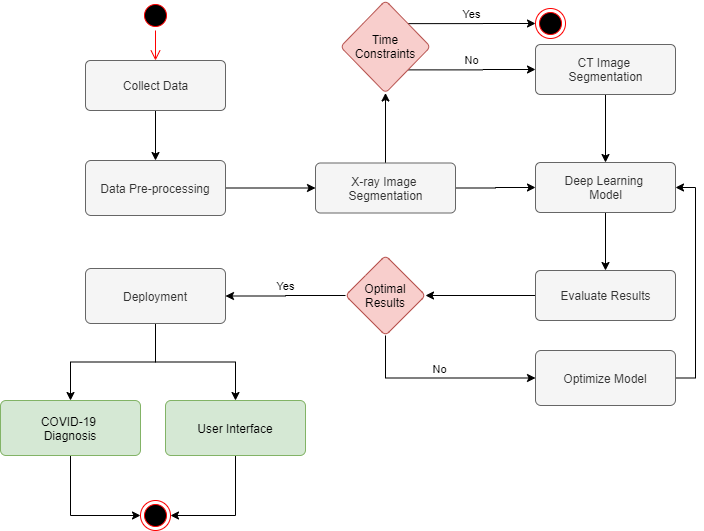
\includegraphics[width=15.5cm]{Images/Implementation Workflow.png}
 \decoRule
 \caption[Implementation Methodology]{Activity Diagram displaying the implementation workflow.}
 \label{fig:Implementation Methodology}
 \end{figure}
 
 \vspace{-2em}
\section{Evaluation Strategy} \label{Evaluation Strategy Section}
Table \ref{tab:Evaluation Strategy} summarizes the methods and strategies used to evaluate each of the Functional Requirements described in Chapter \ref{Requirements Analysis}.

\begin{longtable}{| p{.10\textwidth} | p{.82\textwidth} |} 
\hline
\multicolumn{2}{|c|}{\textbf{Evaluation Strategy}}\\
\hline
\textbf{ID} & \textbf{Description}\\
\hline
FR-1 & \parbox[t]{12.3cm}{\textbf{X-ray Segmentation} \\ The lung segments produced from X-ray scans shall be evaluated based on its capability to identify possible ROIs.}\\\hline
FR-2 & \parbox[t]{12.3cm}{\textbf{CT Segmentation} \\ The lung segments produced from CT scans shall be evaluated based on its capability to identify possible ROIs.}\\\hline
FR-3 & \parbox[t]{12.3cm}{\textbf{COVID-19 Diagnosis using X-ray Scans} \\ The diagnosis results obtained after achieving FR-1 shall be evaluated against various statistical metrics such as Accuracy, Precision and Recall.}\\\hline
FR-4 & \parbox[t]{12.3cm}{\textbf{COVID-19 Diagnosis using CT Scans} \\ The diagnosis results obtained after achieving FR-2 shall be evaluated against various statistical metrics such as Accuracy, Precision and Recall.}\\\hline
FR-5 & \parbox[t]{12.3cm}{\textbf{Visualize Lung Region of Interest's} \\ The ROIs visualized correlates to the observed lung characteristics in COVID-19 patients.} \\\hline
FR-6 & \parbox[t]{12.3cm}{\textbf{Multi-class Diagnosis} \\ The diagnosis results obtained shall be evaluated against various statistical metrics such as Accuracy, Precision and Recall.}\\\hline
FR-7 & \parbox[t]{12.3cm}{\textbf{Web Interface} \\ The user interface developed shall evaluated based on the following metrics, that is, user-friendliness, consistency, familiarity, responsiveness, and intuitiveness\vspace{0.2em}}\\\hline
\caption{Evaluation Strategy}

  \label{tab:Evaluation Strategy}
  \end{longtable}
  
    \vspace{-2em}
\section{Implementation Methodology}
A brief summary of the methodology that would be carried out in semester 2 as well as their evaluation is described in this section.
\subsection{Data Collection}
The two primary sources for collecting open-source anonymized data would be the COVID-19 Kaggle datasets and the scans provided by Cohen et al. \cite{JMD2020} as seen from the literature review. The images obtained shall be separated into X-ray and CT scans separately and furthermore, on the basis of their labels.
\begin{itemize}
    \item \textbf{Testing} - Datasets which correspond to other lung diseases would also be used to analyze the generalizability of the model.
     \item \textbf{Evaluation} - Training would be conducted using  10-fold cross-validation, followed by rigorous verification to prevent the model from either overfitting or underfitting.
\end{itemize}

\subsection{Data Pre-processing}
Before carrying out image segmentation for both X-ray and CT scans, all images in the training dataset shall undergo the same data pre-processing pipeline as per the model's input parameters.
\begin{itemize}
    \item \textbf{Testing} - The model would be tested on images with different dimensions to ensure no input errors are caused.
     \item \textbf{Evaluation} - An input verification technique shall be applied to validate the provided training images before the deep learning workflow commences.
\end{itemize}

\subsection{Image Segmentation}
The provided training images, both X-ray and CT scans shall undergo segmentation such that the ROIs would be highlighted and lead to effective COVID-19 diagnosis
\begin{itemize}
    \item \textbf{Testing} - Multiple image segmentation techniques as suggested by the literature shall be used during the development phase to identify the one that yields the best results.
     \item \textbf{Evaluation} - All models used for experimentation purposes would be documented and the best would be utilized for final demonstration purposes.
\end{itemize}
\subsection{Model Optimization}
As observed in the literature review, multiple studies \cite{CXZ+2020, CYZ+2020, HLR+2020, YHQ+2020, GOM+2020, LLL+2020, CJL+2020, JSB+2020, SFY+2020} indicate variants of the U-Net architecture to be the best suited for CT scan segmentation whereas, for X-rays, variants of ResNet and CNN seem to be ideal as per the research conducted \cite{ZXS+2020, AKP2020, GHT2020, LWA2020}.
\begin{itemize}
    \item \textbf{Testing} - Each of the proposed model variations shall be experimented with for testing purposes, and the results obtained shall be compared to existing literature. 
     \item \textbf{Evaluation} - The results obtained after tweaking the various hyper-parameters for each of the proposed models shall be tracked, thus being able to identify the most optimal set of values.
\end{itemize}


% \section{Research Questions}
% Upon project completion we aim to find answers to the following questions after applying 
% suitable evaluation strategies:

% \begin{itemize}
%   \item Identify whether the ROI's detected by the deep learning model correlates with the lung characteristics observed on COVID-19 patients.
%   \item Compare the results obtained by the deep learning approach with the standard RT-PCR test.
%   \item Feasibility of deploying and utilizing the deep learning model in medical facilities and laboratories for rapid real-time COVID-19 diagnosis.
% \end{itemize}
% % Chapter Template

\chapter{Implementation Methodology and Evaluation Strategy} % Main chapter title

\label{ChapterX} % Change X to a consecutive number; for referencing this chapter elsewhere, use \ref{ChapterX}

%----------------------------------------------------------------------------------------
%	SECTION 1
%----------------------------------------------------------------------------------------

This chapter provides an insight into the project implementation 
workflow, UI wireframe, data collection and processing methodology, 
and concludes with an evaluation strategy.

\section{Implementation Workflow}
The activity diagram displayed below provides a blueprint of the workflow 
that would be followed for the development phase commencing next semester. The wireframe illustrated in Appendix \ref{Wireframe} displays the expected general layout of the COVID-19 diagnosis portal.

\begin{figure}[H]
 \centering
 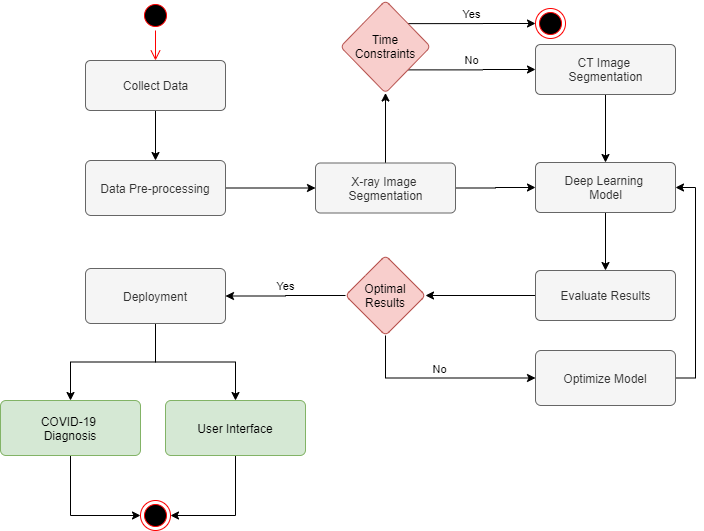
\includegraphics[width=15.5cm, height=7.4cm]{Images/Implementation Workflow.png}
 \decoRule
 \caption[Implementation Methodology]{Activity Diagram displaying the implementation workflow.}
 \label{fig:Implementation Methodology}
 \end{figure}
 
%  \vspace{-2em}
\section{Evaluation Strategy}
Table \ref{Evaluation Strategy} summarizes the methods and strategies used to evaluate each of the Functional Requirements described in Chapter \ref{Requirements Analysis}.

\begin{longtable}{| p{.10\textwidth} | p{.82\textwidth} |} 
\hline
\multicolumn{2}{|c|}{\textbf{Evaluation Strategy}}\\
\hline
\textbf{ID} & \textbf{Description}\\
\hline
FR-1 & \parbox[t]{12.3cm}{\textbf{X-ray Segmentation} \\ The lung segments produced from X-ray scans shall be evaluated based on its capability to identify possible ROIs.}\\\hline
FR-2 & \parbox[t]{12.3cm}{\textbf{CT Segmentation} \\ The lung segments produced from CT scans shall be evaluated based on its capability to identify possible ROIs.}\\\hline
FR-3 & \parbox[t]{12.3cm}{\textbf{COVID-19 Diagnosis using X-ray Scans} \\ The diagnosis results obtained after achieving FR-1 shall be evaluated against various statistical metrics such as Accuracy, Precision and Recall.}\\\hline
FR-4 & \parbox[t]{12.3cm}{\textbf{COVID-19 Diagnosis using CT Scans} \\ The diagnosis results obtained after achieving FR-2 shall be evaluated against various statistical metrics such as Accuracy, Precision and Recall.}\\\hline
FR-5 & \parbox[t]{12.3cm}{\textbf{Visualize Lung Region of Interest's} \\ The ROIs visualized correlates to the observed lung characteristics in COVID-19 patients.} \\\hline
FR-6 & \parbox[t]{12.3cm}{\textbf{Multi-class Diagnosis} \\ The diagnosis results obtained shall be evaluated against various statistical metrics such as Accuracy, Precision and Recall.}\\\hline
FR-7 & \parbox[t]{12.3cm}{\textbf{Web Interface} \\ The user interface developed shall evaluated based on the following metrics, that is, user-friendliness, consistency, familiarity, responsiveness, and intuitiveness\vspace{0.2em}}\\\hline
\caption{Evaluation Strategy}

  \label{tab:Evaluation Strategy}
  \end{longtable}
  
   
\section{Implementation Methodology}
A brief summary of the methodology that would be carried out in semester 2 as well as their evaluation is described in this section.
\subsection{Data Collection}
The two primary sources for collecting open source anonymized data would be the COVID-19 Kaggle datasets and the scans provided by Cohen et al. \cite{JMD2020} as seen from the literature review. The images obtained shall be separated into X-ray and CT scans separately and furthermore, on the basis of their labels.
\begin{itemize}
    \item \textbf{Testing} - Datasets which correspond to other lung diseases would also be used to analyse the generalizability of the model.
     \item \textbf{Evaluation} - Training would be conducted using  10-fold cross validation, followed by rigorous verification to prevent the model from either overfitting or underfitting.
\end{itemize}
\subsection{Data Pre-processing}
Before carrying out image segmentation for both X-ray and CT scans, all images in the training dataset shall undergo the same data pre-processing pipeline as per the model's input parameters.
\begin{itemize}
    \item \textbf{Testing} - The model would be tested on images  with different dimensions to ensure no input errors are caused.
     \item \textbf{Evaluation} - An input verification technique shall be applied to validate the provided training images before the deep learning workflow commences.
\end{itemize}
\subsection{Image Segmentation}
The provided training images, both X-ray and CT scans shall undergo segmentation such that the ROIs would be highlighted and lead to effective COVID-19 diagnosis
\begin{itemize}
    \item \textbf{Testing} - Multiple image segmentation techniques as suggested by the literature shall be used during the development phase to identify the one that yields the best results.
     \item \textbf{Evaluation} - All models used for experimentation purposes would be documented and the best would be utilized for final demonstration purposes.
\end{itemize}
\subsection{Model Optimization}
As observed in the literature review, multiple studies \cite{CXZ+2020, CYZ+2020, HLR+2020, YHQ+2020, GOM+2020, LLL+2020, CJL+2020, JSB+2020, SFY+2020} indicate variants of the U-Net architecture to be the best suited for CT scan segmentation whereas for X-rays, variants of ResNet and CNN seem to be ideal as per the research conducted \cite{ZXS+2020, AKP2020, GHT2020, LWA2020}.
\begin{itemize}
    \item \textbf{Testing} - Each of the proposed model variations shall be experimented with for testing purposes, and the results obtained shall be compared to existing literature. 
     \item \textbf{Evaluation} - The results obtained after tweaking the various hyper-parameters for each of the proposed models shall be tracked, thus being able to identify the most optimal set of values.
\end{itemize}
 
% Chapter Template

\chapter{Project Management} % Main chapter title

\label{ChapterX} % Change X to a consecutive number; for referencing this chapter elsewhere, use \ref{ChapterX}

%----------------------------------------------------------------------------------------
%	SECTION 1
%----------------------------------------------------------------------------------------

This chapter highlights the possible ethical issues and risks that could affect the 
development phase of this project. Furthermore, the proposed development methodology and 
project plan are also included in this section.

\section{Risk Management}
To plan out a balanced and well-thought project development schedule, it is essential 
to take into account the inevitable risks that would occur during the phase and therefore, draw out 
efficient risk mitigation strategies to reduce the impact of the risk on the completion 
of this project. Risk Management comprises of four steps:

\begin{itemize}
    \item \textbf{Risk Identification} - Recognizing various risks and labeling their type as follows.\\
    \vspace{-1em}
    \begin{longtable}
        {| p{.12\textwidth} | p{.12\textwidth} | p{.12\textwidth} | p{.15\textwidth} | p{.14\textwidth} | p{.13\textwidth} |} 
        \hline
        Tools & People & Estimation & Requirements & Organization & Technology \\
        \hline
          \end{longtable}
          \vspace{-1em}
    \item \textbf{Risk Analysis} - Analyzing the probability of risk occurance and their impact if it does infact occur. The following color scheme maps the likelihood and impact of a risk.
\\
    \begin{longtable}
        {| p{.12\textwidth} | p{.12\textwidth} | p{.14\textwidth} |} 
        \hline
        \textbf{Color} & \textbf{Likelihood} & \textbf{Impact}  \\
        \hline
        \cellcolor{red} & High & Catastrophic  \\
        \hline
        \cellcolor{yellow} & Medium& Serious  \\
        \hline
        \cellcolor{green} & Low & Tolerable \\
        \hline
          \end{longtable}
        %   \vspace{-1em}
    \item \textbf{Risk Planning} - Devising risk mitigating strategies and thus reduce its impact on the development phase. 
    These strategies could belong to either \textbf{Avoidance}, \textbf{Minimization}, and \textbf{Contingency} categories respectively. 
    \item \textbf{Risk Monitoring} - Regularly assessing each of the possible risks according to its probability of occurrence.
    \end{itemize}

Table \ref{tab:Risk Analysis} summarizes the identified risks and describes possible mitigating strategies.

\begin{longtable}
    {| p{.5\textwidth} | p{.40\textwidth} | p{.40\textwidth}} 
    \hline
    \multicolumn{3}{|c|}{\textbf{Risk Management}}\\
    \hline
    \multicolumn{1}{|c|}{} & \multicolumn{2}{|c|}{\textbf{Planning and Monitoring}}\\
    \hline
    \multicolumn{1}{|c|}{ \parbox[t]{2.5cm}{\textbf{Risk, Type\\Likelihood, \\Impact}}} & \multicolumn{1}{|c|}{\textbf{Monitoring and Avoidance}} & \multicolumn{1}{|c|}{\textbf{Contingency and Minimization}}\\
    \hline
    \multicolumn{1}{|c|}{ \parbox[t]{2.5cm}{\textbf{Insufficient Data}\\Type: Requirements\\\colorbox{yellow}{\textbf{Likelihood}}\\\colorbox{red}{\textbf{Impact}}}} & \multicolumn{1}{|c|}{\parbox[t]{5.75cm}{\textbf{Monitoring:} Review if the learning model underfits on the training data.\\\textbf{Avoidance:} Explore and store all possible open source COVID-19 data sources such as Kaggle.}} & \multicolumn{1}{|c|}{\parbox[t]{5.75cm}{\textbf{Contingency:} Use datasets for other lung diseases and experiment with Transfer Learning.\\ \textbf{Minimization:} Ensure sufficient data from open source COVID-19 repositories are utilized.}}\\\hline
    \multicolumn{1}{|c|}{ \parbox[t]{2.5cm}{\textbf{Inadequate Computation Power}\\Type: Technology\\\colorbox{green}{\textbf{Likelihood}}\\\colorbox{red}{\textbf{Impact}}}} & \multicolumn{1}{|c|}{\parbox[t]{5.75cm}{\textbf{Monitoring:} Track and ensure reasonable time taken for model training.\\\textbf{Avoidance:} Set up GPU powered deep learning libraries such as Tensorflow-GPU before development phase commences, and ensure sufficient storage  on local machine.\vspace{0.3em}}} & \multicolumn{1}{|c|}{\parbox[t]{5.75cm}{\textbf{Contingency:} Utilize GPU powered cloud computing services such as IBM Cloud or MACS computers. \\ \textbf{Minimization:} Ensure GPU powered deep learning libraries are installed and configured on local machine. \vspace{0.2em}}}\\\hline
    \multicolumn{1}{|c|}{ \parbox[t]{2.5cm}{\textbf{Difficulty in Implementation}\\Type: Requirements\\\colorbox{green}{\textbf{Likelihood}}\\\colorbox{red}{\textbf{Impact}}}} & \multicolumn{1}{|c|}{\parbox[t]{5.75cm}{\textbf{Monitoring:} Rank the proposed models based on ease of implementation, model performance and documentation.\\\textbf{Avoidance:} Thorough literature review and research into the proposed models.}} & \multicolumn{1}{|c|}{\parbox[t]{5.75cm}{\textbf{Contingency:} Utilize alternative models which are well documented and are easily usable. \\ \textbf{Minimization:} Allow sufficient time for project development phase after thorough research into existing studies.}}\\\hline
    \multicolumn{1}{|c|}{ \parbox[t]{2.5cm}{\textbf{Loss of Data}\\Type: Tools\\\colorbox{green}{\textbf{Likelihood}}\\\colorbox{red}{\textbf{Impact}}}} & \multicolumn{1}{|c|}{\parbox[t]{5.75cm}{\textbf{Monitoring:} Perform regular checks on backup sources and processes.\\\textbf{Avoidance:} Set up version control and frequently commit changes to the project repository on GitHub.}} & \multicolumn{1}{|c|}{\parbox[t]{5.75cm}{\textbf{Contingency:} Restart project development phase from scratch. \\ \textbf{Minimization:} Ensure that all phases in development are well documented, and utilize it in an unfortunate scenario of data loss.}}\\\hline
    \multicolumn{1}{|c|}{ \parbox[t]{2.5cm}{\textbf{Slow Project Progression}\\Type: Estimation\\\colorbox{yellow}{\textbf{Likelihood}}\\\colorbox{yellow}{\textbf{Impact}}}} & \multicolumn{1}{|c|}{\parbox[t]{5.75cm}{\textbf{Monitoring:} Ensure that the devised project development schedule is followed precisely. \\\textbf{Avoidance:} Ensure all tools and datasets are set up before commencing development phase and start as early as possible.}} & \multicolumn{1}{|c|}{\parbox[t]{5.75cm}{\textbf{Contingency:} Aim to complete the tasks with the highest priority given limited development time. \\ \textbf{Minimization:} Create a rank based priority list for each of the requirements as per project supervisor's recommendation.}}\\\hline
    \multicolumn{1}{|c|}{ \parbox[t]{2.5cm}{\textbf{Personal Health and Deadlines}\\Type: People\\\colorbox{green}{\textbf{Likelihood}}\\\colorbox{yellow}{\textbf{Impact}}}} & \multicolumn{1}{|c|}{\parbox[t]{5.75cm}{\textbf{Monitoring:} Keep track of the deadlines announced and update the project plan accordingly.\\\textbf{Avoidance:} Achieve weekly targets and ensure that the project supervisor is aware of the announced deadlines.}} & \multicolumn{1}{|c|}{\parbox[t]{5.75cm}{\textbf{Contingency:} Complete tasks as per its importance after discussion with project supervisor. \\ \textbf{Minimization:} Adhere to healthy living practices, follow social distancing protocols and keep flexible plans as per new deadlines.}}\\\hline

    \caption{Risk Analysis}
    
      \label{tab:Risk Analysis}
      \end{longtable}

\section{Project Plan}
The various tasks involved in this project and their proposed completion dates for next semester has 
been illustrated using a Gantt Chart which is displayed in Figure \ref{fig:Project Plan}. TeamGantt was used for 
designing the Gantt Chart, Microsoft Planner would be used to keep track of the weekly 
requirements.

\begin{figure}[H]
 \centering
 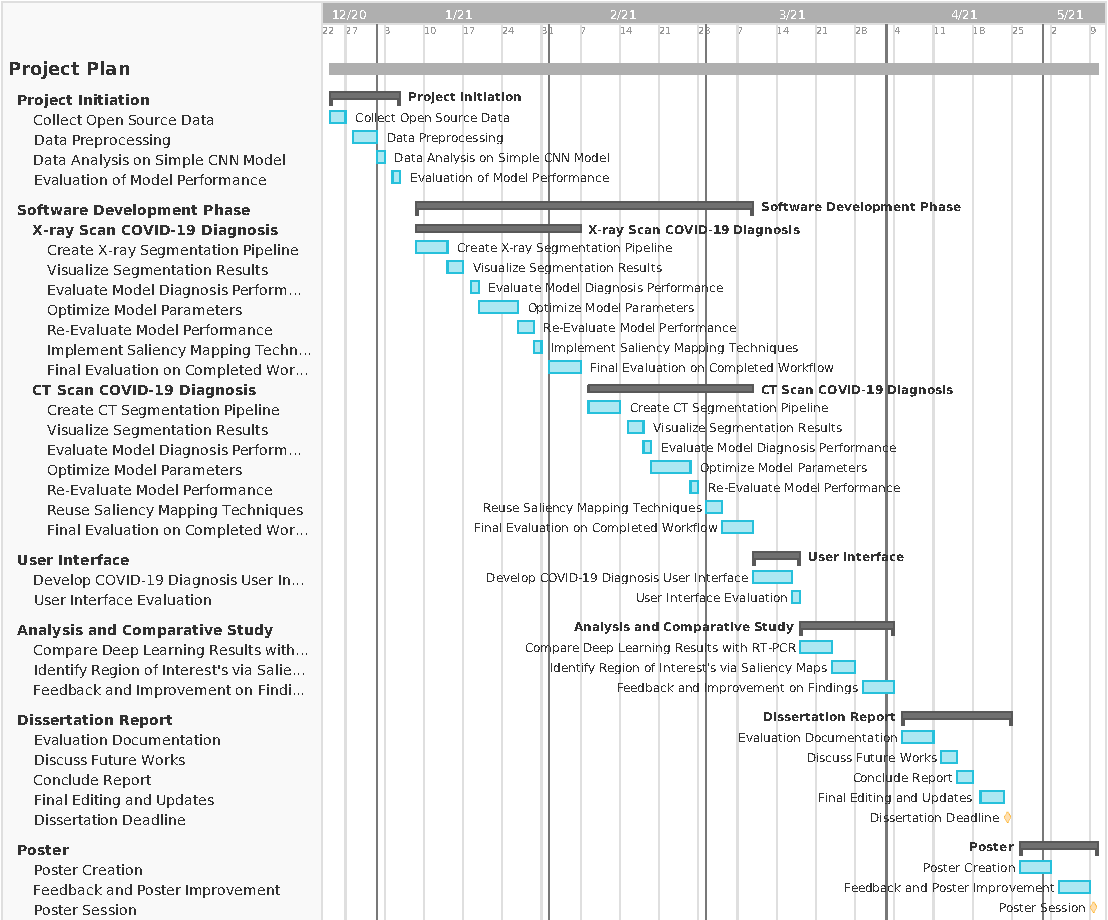
\includegraphics[width=15.5cm]{Images/Project Plan.png}
 \decoRule
 \caption[Project Plan]{Gantt Chart Displaying the proposed Project Plan.}
 \label{fig:Project Plan}
 \end{figure}

\section{Development Methodology}

For this project which involves building a deep learning model 
accompanied by a suitable interface for user interaction, 
an iterative development approach is ideal. \textbf{SCRUM} \cite{SCR}, 
a subset of Agile development methodology proves to be a viable approach. 

Implementing each of the components involved in this project independently 
and adhering to the weekly plan and supervisor's suggestions 
would lead to the deadlines being met and therefore guarantee a successful project completion. 

Further discussion into SCRUM development methodology can be found in Appendix \ref{SCRUM}.

\section{Professional, Legal, Ethical and Social Issues}
\subsection{Professional and Legal Issues}
All research papers discussed in this document are referenced 
accordingly. Any code used from external sources in this project 
shall acknowledge the original authors and would be well documented.
The research papers referenced in this project are either open source 
or have been granted access. The code used for this project shall be 
open source and would be published under the MIT License.

\subsection{Ethical and Social Issues}
No human subjects are involved in this dissertation project. The 
datasets used would be open source and will not 
contain any personal user information and therefore anonymized. Furthermore, all data utilized in this 
project shall be referenced. This project shall not cause any harm to the 
surrounding environment or to any observers.

This project aims to develop a fully automated and rapid COVID-19 diagnosis 
mechanism that reduces virus exposure between patients and 
medical professionals. Through this project, medical professionals 
would receive real-time COVID-19 diagnosis from the provided lung scans, and thus, would be able to rank them based on severity, 
and ultimately save lives.
 


%----------------------------------------------------------------------------------------
%	THESIS CONTENT - APPENDICES
%----------------------------------------------------------------------------------------

\appendix % Cue to tell LaTeX that the following "chapters" are Appendices

% Include the appendices of the thesis as separate files from the Appendices folder
% Uncomment the lines as you write the Appendices

% Chapter Template

\chapter{Requirements Analysis and Evaluation Strategy} % Main chapter title
\label{Requirements Analysis} % Change X to a consecutive number; for referencing this chapter elsewhere, use \ref{ChapterX}

%----------------------------------------------------------------------------------------
%	SECTION 1
%----------------------------------------------------------------------------------------

This chapter provides an insight into the project requirements followed by demonstrating the project implementation workflow, UI wireframe, data collection, and processing methodology, and concludes with an evaluation strategy.

\section{Requirements Analysis}
This section identifies and outlines the functional and non-functional requirements pertaining to this project. The priority 
of each of these requirements are ranked according to the MSCW prioritization technique. The following color-scheme 
indicates the respective ranking order:

\begin{itemize}
  \item \colorbox{green}{\textbf{Must Have (M)}} - These requirements are fundamental to achieve the aim of this project.
  \item \colorbox{cyan}{\textbf{Should Have (S)}} - These requirements are important to the project but not vital and could be achieved in the long run.
  \item \colorbox{yellow}{\textbf{Could Have (C)}} - These requirements are not fundamental to achieve the aim of this project but would be an added benefit if accomplished.
  \item \colorbox{pink}{\textbf{Want To Have (W)}} - These requirements would be prioritized in later releases of the project.
\end{itemize}

\subsection{Functional and Non-Functional Requirements}
The Functional Requirements (FR's) describes the essential components, purpose, and objectives of this project.
Table \ref{tab:Functional Requirements} tabulates the FR's along with a brief description for the same and its priority according to MSCW prioritization technique. An evaluation 
for each of these functional requirements is specified in section \ref{Evaluation Strategy Section}.

% \subsection{Non-Functional Requirements}
Non-Functional Requirements (NFR's) emphasizes the system's operation which includes its performance, usability, portability, and so on. Table \ref{tab:Non-Functional Requirements} tabulates each of these NFR's and applies the MSCW prioritization technique.

\begin{longtable}{| p{.10\textwidth} | p{.70\textwidth} | p{.10\textwidth} |} 
\hline
\multicolumn{3}{|c|}{\textbf{Functional Requirements}}\\
\hline
\textbf{ID} & \textbf{Description} & \textbf{Priority}  \\
\hline
FR-1 & \textbf{X-ray Segmentation}  & \cellcolor{green}\textbf{M} \\ &  The system shall be able to accept and segment X-ray scans. & \cellcolor{green} \\ \hline 
FR-2 & \textbf{CT Segmentation}  & \cellcolor{cyan}\textbf{S} \\ &  The system shall be able to accept and segment CT scans. & \cellcolor{cyan} \\ \hline 
FR-3 & \textbf{COVID-19 Diagnosis using X-ray Scans}  & \cellcolor{green}\textbf{M} \\ & The system shall be able to classify positive COVID-19 patients from others given test X-ray scans & \cellcolor{green} \\ \hline 
FR-4 & \textbf{COVID-19 Diagnosis using CT Scans}  & \cellcolor{cyan}\textbf{S} \\ &  The system shall be able to classify positive COVID-19 patients from others given test CT scans. & \cellcolor{cyan} \\ \hline
FR-5 & \textbf{Visualize Lung Region of Interest's}  & \cellcolor{green}\textbf{M} \\ &  The system shall be able to interpret and visualize classification results by highlighting lung ROIs. & \cellcolor{green} \\ \hline 
FR-6 & \textbf{Multi-class Diagnosis}  & \cellcolor{pink}\textbf{W} \\ &  The system shall be able to differentiate COVID-19 and Pneumonia (Viral or Bacterial) patients. & \cellcolor{pink} \\ \hline 
FR-7 & \textbf{Web Interface}  & \cellcolor{cyan}\textbf{S} \\ &  The system shall have an interface which presents diagnosis results after segmentation for visualization and analysis purposes. & \cellcolor{cyan} \\ \hline

% \multirowcell{2}{FR2} & 70 COVID-19 & \cellcolor{green} \\ & Others & \multirowcell{-2}{*}{ \cellcolor{green}S}\\ \hline
\caption{Functional Requirements}

  \label{tab:Functional Requirements}
  \end{longtable}

%   \begin{longtable}{| p{.10\textwidth} | p{.70\textwidth} | p{.10\textwidth} |} 
%     \hline
%     \multicolumn{3}{|c|}{\textbf{User Functional Requirements}}\\
%     \hline
%     \textbf{ID} & \textbf{Description} & \textbf{Priority}  \\
%     \hline
%     U-FR-1 & \textbf{Input X-ray Scans}  & \cellcolor{green}\textbf{M} \\ & The user shall be able to provide X-ray scan images as input for COVID-19 diagnosis. & \cellcolor{green} \\ \hline 
%     U-FR-2 & \textbf{Input CT Scans}  & \cellcolor{cyan}\textbf{S} \\ &   The user shall be able to provide CT scan images as input for COVID-19 diagnosis. & \cellcolor{cyan} \\ \hline 
%     U-FR-3 & \textbf{Save Classification Results}  & \cellcolor{green}\textbf{M} \\ & The user shall be able to save and interact with the classification results which highlights the lung ROI's. & \cellcolor{green} \\ \hline 

%     % \multirowcell{2}{FR2} & 70 COVID-19 & \cellcolor{green} \\ & Others & \multirowcell{-2}{*}{ \cellcolor{green}S}\\ \hline
%     \caption{User Functional Requirements}
    
%       \label{tab:User Functional Requirements}
%       \end{longtable}

\vspace{5em}
% \\\\
\begin{longtable}{| p{.10\textwidth} | p{.70\textwidth} | p{.10\textwidth} |} 
  
  \hline
  \multicolumn{3}{|c|}{\textbf{Non-Functional Requirements}}\\
  \hline
  \textbf{ID} & \textbf{Description} & \textbf{Priority}  \\
  \hline
  NFR-1 & \textbf{Environment}  & \cellcolor{yellow}\textbf{C} \\ & The system shall be deployed on a cloud platform such as IBM Cloud. & \cellcolor{yellow} \\ \hline 
  NFR-2 & \textbf{User Interface}  & \cellcolor{cyan}\textbf{S} \\ &   The system shall have an intuitive and user-friendly interface evaluated via a System Usability Study where the user can input scans and receive diagnosis results which could be confirmed by a medical professional. & \cellcolor{cyan} \\ \hline 
  NFR-3 & \textbf{Extensibility}  & \cellcolor{cyan}\textbf{S} \\ & The system shall be flexible to extensions, this includes bug fixes, updated features and performance improvement.& \cellcolor{cyan} \\ \hline 
  NFR-4 & \textbf{Version Control}  & \cellcolor{green}\textbf{M} \\ & All versions of the code shall be published on GitHub which enables version control and be open source.& \cellcolor{green} \\ \hline 
  NFR-5 & \textbf{Documentation}  & \cellcolor{green}\textbf{M} \\ & The code shall include relevant comments and contain an instructions guide to setup the environment and run the code. & \cellcolor{green} \\ \hline 
  NFR-6 & \textbf{Modular Programming}  & \cellcolor{cyan}\textbf{S} \\ & The program functionality shall be separated into independent components to emphasize the scalability of software.& \cellcolor{cyan} \\ \hline 
  NFR-7 & \textbf{Reusability}  & \cellcolor{yellow}\textbf{C} \\ & The code developed shall be reusable by other researchers and developers. & \cellcolor{yellow} \\ \hline 

  % \multirowcell{2}{FR2} & 70 COVID-19 & \cellcolor{green} \\ & Others & \multirowcell{-2}{*}{ \cellcolor{green}S}\\ \hline
  \caption{Non-Functional Requirements}
  
    \label{tab:Non-Functional Requirements}
    \end{longtable}


% This chapter provides an insight into the project implementation 
% workflow, UI wireframe, data collection, and processing methodology, 
% and concludes with an evaluation strategy.
\vspace{-2em}
\section{Implementation Workflow}
The activity diagram displayed in Figure \ref{fig:Implementation Methodology} provides a blueprint of the workflow that would be followed for the development phase commencing next semester. 

% The wireframe illustrated in Appendix \ref{Wireframe} displays the expected general layout of the COVID-19 diagnosis portal.

\begin{figure}[H]
 \centering
 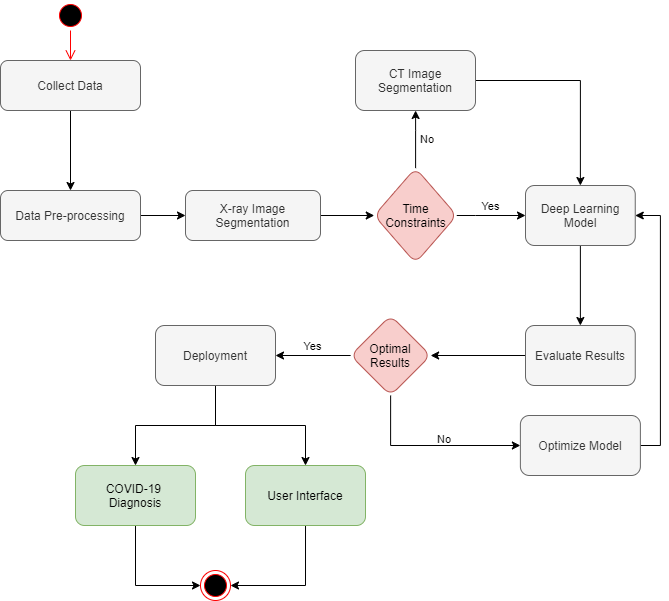
\includegraphics[width=15.5cm, height=11.5cm]{Images/activityDiagram.png}
%  \decoRule
 \caption[Implementation Methodology]{Activity Diagram displaying the implementation workflow.}
 \label{fig:Implementation Methodology}
 \end{figure}
 
 \vspace{-2em}
\section{Evaluation Strategy} \label{Evaluation Strategy Section}
Table \ref{tab:Evaluation Strategy} summarizes the methods and strategies used to evaluate each of the Functional Requirements described in Chapter \ref{Requirements Analysis}.

\begin{longtable}{| p{.10\textwidth} | p{.82\textwidth} |} 
\hline
\multicolumn{2}{|c|}{\textbf{Evaluation Strategy}}\\
\hline
\textbf{ID} & \textbf{Description}\\
\hline
FR-1 & \parbox[t]{12.3cm}{\textbf{X-ray Segmentation} \\ The lung segments produced from X-ray scans shall be evaluated based on its capability to identify possible ROIs.}\\\hline
FR-2 & \parbox[t]{12.3cm}{\textbf{CT Segmentation} \\ The lung segments produced from CT scans shall be evaluated based on its capability to identify possible ROIs.}\\\hline
FR-3 & \parbox[t]{12.3cm}{\textbf{COVID-19 Diagnosis using X-ray Scans} \\ The diagnosis results obtained after achieving FR-1 shall be evaluated against various statistical metrics such as Accuracy, Precision and Recall.}\\\hline
FR-4 & \parbox[t]{12.3cm}{\textbf{COVID-19 Diagnosis using CT Scans} \\ The diagnosis results obtained after achieving FR-2 shall be evaluated against various statistical metrics such as Accuracy, Precision and Recall.}\\\hline
FR-5 & \parbox[t]{12.3cm}{\textbf{Visualize Lung Region of Interest's} \\ The ROIs visualized correlates to the observed lung characteristics in COVID-19 patients.} \\\hline
FR-6 & \parbox[t]{12.3cm}{\textbf{Multi-class Diagnosis} \\ The diagnosis results obtained shall be evaluated against various statistical metrics such as Accuracy, Precision and Recall.}\\\hline
FR-7 & \parbox[t]{12.3cm}{\textbf{Web Interface} \\ The user interface developed shall evaluated based on the following metrics, that is, user-friendliness, consistency, familiarity, responsiveness, and intuitiveness\vspace{0.2em}}\\\hline
\caption{Evaluation Strategy}

  \label{tab:Evaluation Strategy}
  \end{longtable}
  
    \vspace{-2em}
\section{Implementation Methodology}
A brief summary of the methodology that would be carried out in semester 2 as well as their evaluation is described in this section.
\subsection{Data Collection}
The two primary sources for collecting open-source anonymized data would be the COVID-19 Kaggle datasets and the scans provided by Cohen et al. \cite{JMD2020} as seen from the literature review. The images obtained shall be separated into X-ray and CT scans separately and furthermore, on the basis of their labels.
\begin{itemize}
    \item \textbf{Testing} - Datasets which correspond to other lung diseases would also be used to analyze the generalizability of the model.
     \item \textbf{Evaluation} - Training would be conducted using  10-fold cross-validation, followed by rigorous verification to prevent the model from either overfitting or underfitting.
\end{itemize}

\subsection{Data Pre-processing}
Before carrying out image segmentation for both X-ray and CT scans, all images in the training dataset shall undergo the same data pre-processing pipeline as per the model's input parameters.
\begin{itemize}
    \item \textbf{Testing} - The model would be tested on images with different dimensions to ensure no input errors are caused.
     \item \textbf{Evaluation} - An input verification technique shall be applied to validate the provided training images before the deep learning workflow commences.
\end{itemize}

\subsection{Image Segmentation}
The provided training images, both X-ray and CT scans shall undergo segmentation such that the ROIs would be highlighted and lead to effective COVID-19 diagnosis
\begin{itemize}
    \item \textbf{Testing} - Multiple image segmentation techniques as suggested by the literature shall be used during the development phase to identify the one that yields the best results.
     \item \textbf{Evaluation} - All models used for experimentation purposes would be documented and the best would be utilized for final demonstration purposes.
\end{itemize}
\subsection{Model Optimization}
As observed in the literature review, multiple studies \cite{CXZ+2020, CYZ+2020, HLR+2020, YHQ+2020, GOM+2020, LLL+2020, CJL+2020, JSB+2020, SFY+2020} indicate variants of the U-Net architecture to be the best suited for CT scan segmentation whereas, for X-rays, variants of ResNet and CNN seem to be ideal as per the research conducted \cite{ZXS+2020, AKP2020, GHT2020, LWA2020}.
\begin{itemize}
    \item \textbf{Testing} - Each of the proposed model variations shall be experimented with for testing purposes, and the results obtained shall be compared to existing literature. 
     \item \textbf{Evaluation} - The results obtained after tweaking the various hyper-parameters for each of the proposed models shall be tracked, thus being able to identify the most optimal set of values.
\end{itemize}


% \section{Research Questions}
% Upon project completion we aim to find answers to the following questions after applying 
% suitable evaluation strategies:

% \begin{itemize}
%   \item Identify whether the ROI's detected by the deep learning model correlates with the lung characteristics observed on COVID-19 patients.
%   \item Compare the results obtained by the deep learning approach with the standard RT-PCR test.
%   \item Feasibility of deploying and utilizing the deep learning model in medical facilities and laboratories for rapid real-time COVID-19 diagnosis.
% \end{itemize}
% Appendix Template

\chapter{COVID-19 Lung Characteristics} \label{COVID-19 Lung Characteristics} % Change X to a consecutive letter; for referencing this appendix elsewhere, use \ref{AppendixX}


\section*{Additional Study on COVID-19 Patients}

Morales et al. conducted a systematic literature review with meta-analysis 
of the imaging features of COVID-19 also observed similar lung characteristics 
such as GGO's from X-ray scans from patients diagnosed with COVID-19 from 
multiple studies \cite{RAJ+2020}, the results are tabulated in Table \ref{tab:Chest X-ray Review Results}.
\vspace{1em}

\begin{longtable}{| p{.27\textwidth} | p{.20\textwidth} | p{.20\textwidth} | p{.20\textwidth} |} 
    
    \hline
\textbf{Study} & \textbf{Unilateral Pneumonia} & \textbf{Bilateral Pneumonia} & \textbf{Ground-glass Opacity} \\
\hline

Huang et al. \cite{CYX+2020} & - & 40 (97.6\%) & 12 (29.3\%)\\ \hline
Chen et al. \cite{CNM+2020} & 25 (25.3\%) & 74 (74.7\%) & 14 (14.1\%)\\ \hline
Wang et al. \cite{WDC+2020} & 0 (0\%)& 138 (100.0\%) & 138 (100.0\%)\\ \hline
Liu et al. \cite{LKY+2020} & - & 36 (26.3\%) & 55 (40.1\%)\\ \hline
Chang et al. \cite{CML+2020} & 1 (7.7\%)& - & 6 (46.2\%)\\ \hline
Pan et al. \cite{PYH+2020} & - & 38 (60.3\%) & 14 (22.2\%)\\ \hline
Zhang et al. \cite{ZMX+2020} & 2 (22.2\%)& 5 (55.6\%)& 7 (77.8\%)\\ \hline

 \caption{Chest X-ray imaging characteristics from multiple studies}

    \label{tab:Chest X-ray Review Results}
    \end{longtable}
\vspace{-1em}
% Appendix Template

\chapter{The COVID-19 Pandemic Era} \label{The COVID-19 Pandemic Era} % Change X to a consecutive letter; for referencing this appendix elsewhere, use \ref{AppendixX}


\section*{Rise of the Global Pandemic}

COVID-19 which is now officially declared as a global pandemic by the WHO was 
initially discovered in late 2019 emerging from Wuhan, People’s Republic of China.
A media statement was released by the Wuhan Municipal Health Commission confirming
multiple cases of "Viral Pneumonia from an unknown cause" on December 31$^{st}$ 2019 \cite{WMC2020}.

On January 7$^{th}$ 2020, this unknown disease was identified as the novel coronavirus by the WHO.
Three days later, the first known death caused by the coronavirus was reported \cite{WHOa2020}. The 
spread of the virus continued rapidly within China and on January 20$^{th}$ 2020, WHO reports 
the first confirmed cases outside China in Thailand, Japan, and South Korea. The very next day 
The United States reports its first confirmed coronavirus case \cite{EDW2020}. 

Following these set of events saw the introduction of quarantine protocols via lockdowns. 
Starting with Wuhan, many other cities across the world also adopted the same orders to 
suspend the spread of the coronavirus. This prompted the WHO to declare the outbreak a global public health emergency \cite{EDWa2020}. 

Within the span of a month, the death toll from COVID-19 surpassed that of SARS 
and the WHO gives the official name for the disease caused by the coronavirus "COVID-19" \cite{MCM2020}. 
The adverse effects of COVID-19 on various industries and the stock market began to 
show.

\begin{figure}[th]
\centering
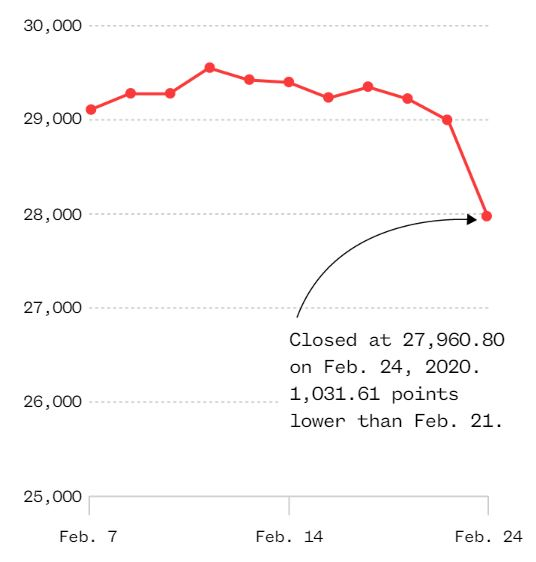
\includegraphics[height=7cm]{Images/stockMarket.JPG}
% \decoRule
\caption[Dow Jones]{Dow Jones Industrial Average experienced the worst day in two years. \cite{WBY2020}}
\label{fig:Dow Jones}
\end{figure}

Travel bans, high-profile event cancellations and activation of emergency funds were 
implemented across different countries as the number of positive cases rose above 100,000 \cite{SHA2020}.

Due to the rapid spread of the virus worldwide, on March 11$^{th}$ 2020, the WHO declares the coronavirus 
outbreak as a global pandemic \cite{JAS2020}. Over the next few months, nationwide 
lockdowns were enforced in countries such as The United Kingdom, India, South Africa, Italy, Belgium, and so on.

At the end of March 2020, The United States coronavirus cases officially surpassed China, with the former 
reporting 82,474 cases and the latter 81,961 cases.

\begin{figure}[H]
    \centering
    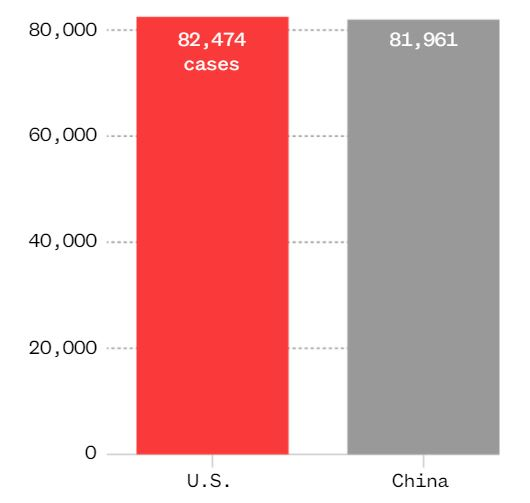
\includegraphics[height=7cm]{Images/usCases.JPG}
    % \decoRule
    \caption[COVID-19 Cases]{COVID-19 cases comparison between The United States and China \cite{GIV2020}}
    \label{fig:COVID-19 Cases Comparison}
    \end{figure}

On April 2$^{nd}$ 2020, the number of coronavirus cases worldwide surpassed 1 million with the number of deaths exceeding 51,000 \cite{PHI2020}. 
The number of positive cases doubled in April and this trend continued to follow for the next few months were as of 
October 2$^{nd}$ 2020, the total number of worldwide COVID-19 cases stand at 34,312,510, and the death toll surpassing over a million, to be precise 1,023,243 \cite{GGN2020}. 

Among the countries affected by COVID-19, The United States, India and Brazil share the 
highest percentages of positive cases.  

\begin{figure}[H]
    \centering
    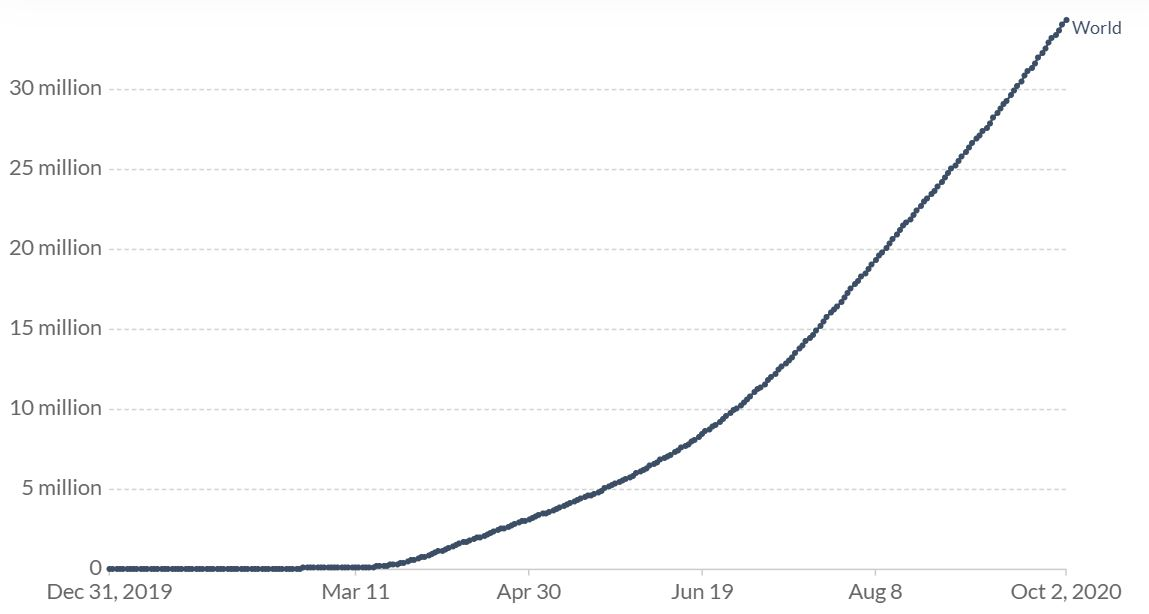
\includegraphics[width=15cm, height=6cm]{Images/totalCases.JPG}
    % \decoRule
    \caption[Total COVID-19 Cases]{Cumulative confirmed COVID-19 cases \cite{ECDC2020}}
    \label{fig:Total COVID-19 Cases}
    \end{figure}

   
\begin{figure}[H]
    \centering
    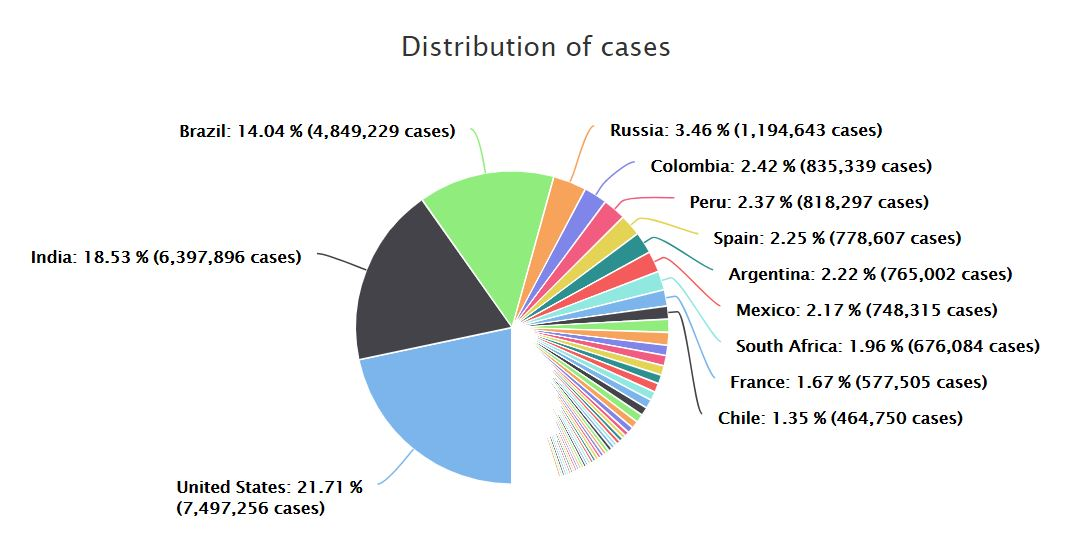
\includegraphics[width=15cm]{Images/casesDist.JPG}
    % \decoRule
    \caption[Distribution of COVID-19 Cases]{Country wise distribution of COVID-19 cases \cite{WMR2020}}
    \label{fig:COVID-19 Cases Country Wise Distribution}
    \end{figure}

    As we have now seen the major trends and events that took place in the rapid spread of COVID-19, it is upon us to work together as a community, follow the recommendations suggested by national and international healthcare agencies through which we would be able to overcome this pandemic and successfully curb the spread of the virus.
% Appendix Template

\chapter{COVID-19 Lung Characteristics} \label{COVID-19 Lung Characteristics} % Change X to a consecutive letter; for referencing this appendix elsewhere, use \ref{AppendixX}


\section*{Additional Study on COVID-19 Patients}

Morales et al. conducted a systematic literature review with meta-analysis 
of the imaging features of COVID-19 also observed similar lung characteristics 
such as GGO's from X-ray scans from patients diagnosed with COVID-19 from 
multiple studies \cite{RAJ+2020}, the results are tabulated in Table \ref{tab:Chest X-ray Review Results}.
\vspace{1em}

\begin{longtable}{| p{.27\textwidth} | p{.20\textwidth} | p{.20\textwidth} | p{.20\textwidth} |} 
    
    \hline
\textbf{Study} & \textbf{Unilateral Pneumonia} & \textbf{Bilateral Pneumonia} & \textbf{Ground-glass Opacity} \\
\hline

Huang et al. \cite{CYX+2020} & - & 40 (97.6\%) & 12 (29.3\%)\\ \hline
Chen et al. \cite{CNM+2020} & 25 (25.3\%) & 74 (74.7\%) & 14 (14.1\%)\\ \hline
Wang et al. \cite{WDC+2020} & 0 (0\%)& 138 (100.0\%) & 138 (100.0\%)\\ \hline
Liu et al. \cite{LKY+2020} & - & 36 (26.3\%) & 55 (40.1\%)\\ \hline
Chang et al. \cite{CML+2020} & 1 (7.7\%)& - & 6 (46.2\%)\\ \hline
Pan et al. \cite{PYH+2020} & - & 38 (60.3\%) & 14 (22.2\%)\\ \hline
Zhang et al. \cite{ZMX+2020} & 2 (22.2\%)& 5 (55.6\%)& 7 (77.8\%)\\ \hline

 \caption{Chest X-ray imaging characteristics from multiple studies}

    \label{tab:Chest X-ray Review Results}
    \end{longtable}
\vspace{-1em}
% Appendix Template

\chapter{Automated Diagnosis Workflow} \label{Automated Diagnosis Workflow} % Change X to a consecutive letter; for referencing this appendix elsewhere, use \ref{AppendixX}


\section*{AI Powered Medical Scanning}

Chest X-ray and CT scans are the primary screening mechanisms for
diagnosing COVID-19. The limitation to these being the viral 
exposure between the technician and the patient, as assistance 
is required to perfect patient positioning for these scans to 
yield satisfactory results. Therefore, an automated and 
contact-less workflow is the need of the hour.

Modern CT and X-ray systems include cameras to allow 
technicians to remotely monitor the patient. But especially 
since the outbreak of the pandemic, this would not be 
sufficient as technicians would not be able to determine 
scanning parameters such as scan range \cite{SFJ+2020}.

Fortunately, a fully automated scanning workflow is indeed possible 
through AI. Patient pose and shape could be acquired via 
visual sensors such as RGB, Time-of-Flight (TOF) pressure imaging or 
thermal (FIR) cameras. Therefore, optimal scanning parameters could be 
determined \cite{UIH2020, SVK+2017, SVY+2017, SIE2020, LJU+2020, MAR2020, AFA+2020, SIE(2)2020}.

Through this automated scanning workflow, radiation exposure 
can be reduced significantly as well as increasing the overall efficiency of the 
diagnosis procedure \cite{WYX+2020}. Especially during this period of the pandemic, using 
the same workflow would prevent virus exposure between technicians or 
medical practitioners and patients.
\\
\begin{figure}[H]
    \centering
    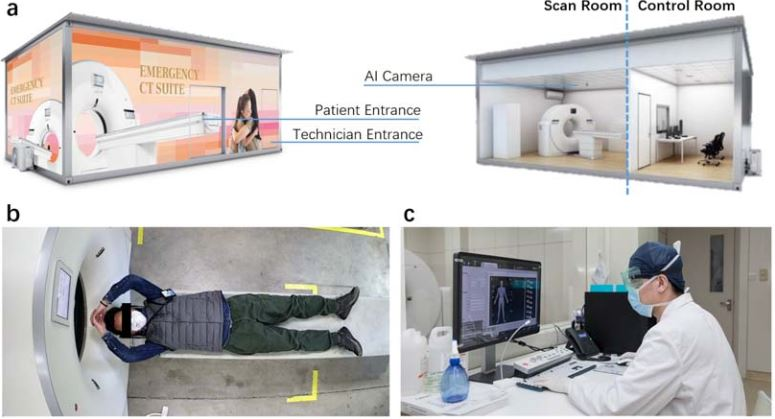
\includegraphics{Images/AutomatedCTScan.JPG}
    % \decoRule
    \caption[Mobile CT Platform]{AI-empowered automated image acquisition workflow \cite{SFJ+2020}.}
    \label{fig:Mobile CT Platform}
    \end{figure}

Utilizing this workflow we can procure high-quality X-ray and CT scans suitable for segmentation, but more importantly, we can ensure the safety of both patients and technicians by reducing the radiation and virus exposure respectively. 
% To carry out the automated diagnosis process, segmentation of the 
% lung CT or X-ray scans are a vital pre-requisite in order to identify the regions of interest (ROIs). The former produces 
% high-quality 3D images for detecting COVID-19 whereas the latter involves 
% the ribs being projected onto soft-tissues in 2D. As a result, image segmentation 
% in X-ray scans is more challenging as compared to CT scans. But on the other hand, 
% X-ray scans are more widely accessible in medical facilities all across the world 
% and are usually the first imaging modality used on patients suspected of COVID-19.

% Keeping in mind these limitations, in the next two subsections review the
% image segmentation techniques using deep learning for both CT and X-rays respectively and 
% discuss the results obtained.

% Appendix Template

\chapter{SCRUM} \label{SCRUM} % Change X to a consecutive letter; for referencing this appendix elsewhere, use \ref{AppendixX}


\section*{SCRUM Development Methodology}

SCRUM involves building software iteratively coupled with a continuous integration 
and development pipeline if set up, this enables frequent feedback 
from the project supervisor. This development methodology allows us to 
perform weekly increments where a reasonable part of the functionality is 
developed or modified and these updates could be reviewed by the project 
supervisor. Therefore, it would be easier to detect and mitigate risks involved such as 
slow progression in model development or misinterpretation of the project requirements.

\begin{figure}[th]
    \centering
    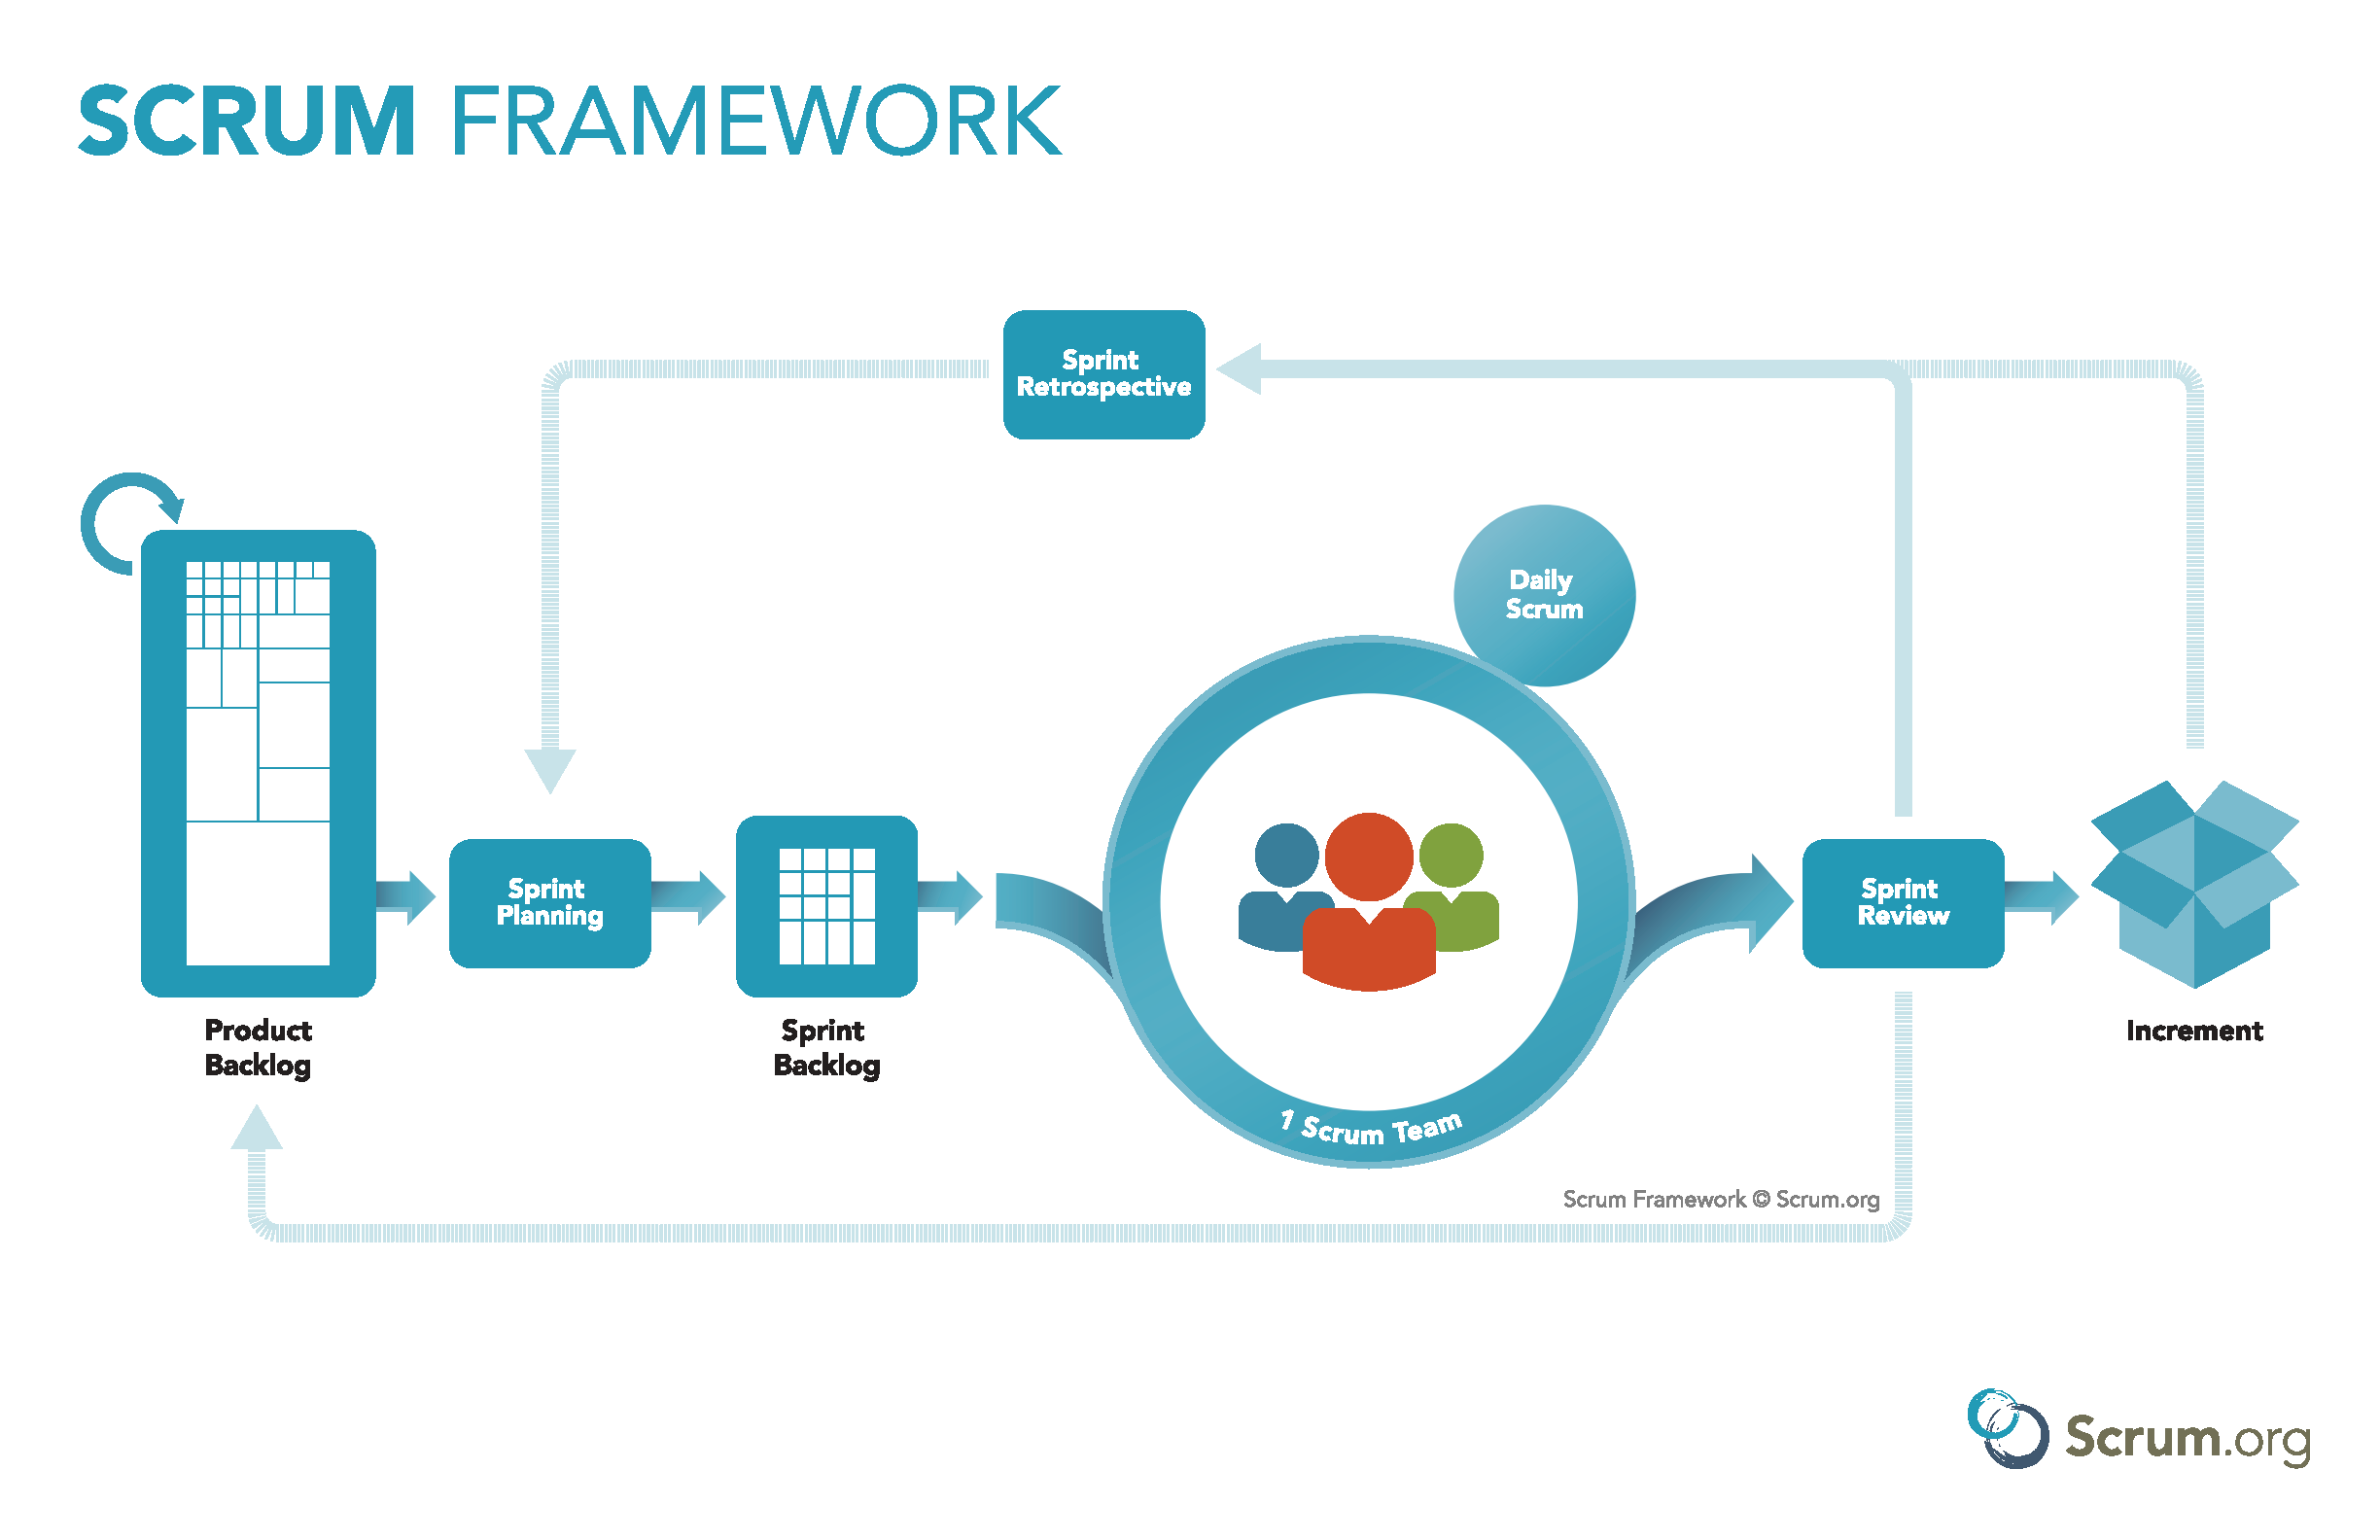
\includegraphics[width=15cm, height=6cm]{Images/SCRUM.png}
    \decoRule
    \caption[SCRUM]{SCRUM Development Methodology \cite{SFP}}
    \label{fig:SCRUM}
    \end{figure}

%----------------------------------------------------------------------------------------
%	BIBLIOGRAPHY
%----------------------------------------------------------------------------------------

\printbibliography[heading=bibintoc]
%\bibliographystyle{IEEEtran}
%----------------------------------------------------------------------------------------

\end{document}  
